\documentclass[12pt, a4paper]{article}

\usepackage[utf8]{inputenc}
\usepackage[italian]{babel}
\usepackage{geometry}
\geometry{a4paper, top=3cm, bottom=3cm, left=2.5cm, right=2.5cm}
\usepackage{tabularx}
\usepackage{booktabs}
\usepackage{hyperref}
\usepackage{eurosym}
\usepackage{graphicx}
\usepackage{titlesec}
\usepackage[figure,table]{totalcount}
\usepackage{fancyhdr}
\usepackage{adjustbox}
\usepackage{extramarks}
\usepackage{makecell}
\usepackage{float}
\usepackage[skip=10pt plus 2pt, indent=5pt]{parskip}
\usepackage{hyperref}
\usepackage{xltabular}
\usepackage{array}

\newcolumntype{D}{>{\hsize=1.6\hsize\raggedright\arraybackslash}X}
\newcolumntype{F}{>{\hsize=0.4\hsize\raggedright\arraybackslash}X}
\newcommand{\urlglossario}{https://skynetunigroup.github.io/Code_Guardian/Documentazione/RTB/glossario_v0.2.pdf} % Da aggiornare con nuove versioni
\newcommand{\glo}[2]{\href{\urlglossario\#nameddest=#2}{#1\textsubscript{G}}}

\pagestyle{fancy}
\fancyhf{}
\setlength{\headheight}{35pt}

\hypersetup{
    pdftitle={Analisi dei requisiti},
    colorlinks=true,
    linkcolor=black,
    filecolor=magenta,      
    urlcolor=blue,
}

\newcommand{\doctitle}{Analisi dei Requisiti} % Sostituisci con il titolo reale

% --- INTESTAZIONE (HEADER) ---
\lhead{\nouppercase{\firstleftmark}}
\rhead{\adjustbox{valign=m}{
\includegraphics[height=1cm]{logo_skynet_dark.png}}}

% --- PIÈ DI PAGINA (FOOTER) ---
\lfoot{\doctitle} 
\rfoot{\thepage} 

% Linee di separazione
\renewcommand{\headrulewidth}{0.4pt} % Linea sotto l'intestazione
\renewcommand{\footrulewidth}{0.4pt} % Linea sopra il piè di pagina

\begin{document}
% ==========================================
% FRONTESPIZIO
% ==========================================
\begin{titlepage}
    \centering
    
\includegraphics[width=0.5\linewidth]{logo_skynet_dark.png}
    
    {\Large Gruppo SkyNet}\\
   
    {\normalsize \href{mailto:skynetunigroup@gmail.com}{skynetunigroup@gmail.com}}
    \vspace*{1.5cm}
    
    {\Huge \textbf{\doctitle}} \\
    
    \vspace{3cm}
    
    % Tabella Informazioni Documento, sostituire con il contenuto reale
    \begin{table}[h]
        \centering
        \renewcommand{\arraystretch}{1.5}
        \begin{tabularx}{\textwidth}{|l|X|}
            \hline
            \textbf{Versione} & \textit{0.13.0} \\ \hline
    
            \textbf{Uso} & \textit{Esterno} \\ \hline
            \textbf{Destinatari} & \textit{Prof. Tullio Vardanega, Prof. Riccardo Cardin} \\ \hline
            \textbf{Redattori} & \textit{Sara Ristovic, Marco Barbiero, Dario Pirrone} \\ \hline
            \textbf{Verifica} & \textit{Dario Pirrone, Marco Barbiero, Samuele Bertin, Edoardo Granziero} \\ \hline
            \textbf{Approvazione} & \textit{Samuele Bertin, Dario Pirrone, Andrea Fistarol, Edoardo Granziero, Sara Ristovic} \\ \hline

        \end{tabularx}
    \end{table}
    
    \vfill
\end{titlepage}
\stepcounter{page}

\newpage



% ==========================================
% REGISTRO DELLE VERSIONI
% ==========================================
\section*{Versioni del documento}
\markboth{Versioni del documento}{}
\renewcommand{\arraystretch}{1.3}

\begin{xltabular}{\textwidth}{|c|c|>{\raggedright\arraybackslash}X|l|l|}
    \hline
    \textbf{Ver.} & \textbf{Data} & \textbf{Descrizione} & \textbf{Autore} & \textbf{Verificatore} \\ \hline
    \endfirsthead 
    
    \hline
    \textbf{Ver.} & \textbf{Data} & \textbf{Descrizione} & \textbf{Autore} & \textbf{Verificatore} \\ \hline
    \endhead 
    

    0.13.0 & 2026/06/08 & Aggiunti diagrammi UML per Agente OWASP e Agente Changelog & Dario Pirrone & Edoardo Granziero \\ \hline 
    0.12.1 & 2026/06/06 & Modificata numerazione UC e requisiti & Dario Pirrone & Edoardo Granziero \\ \hline 
    0.12.0 & 2026/06/05 & Modifiche varie a UC e ai requisiti a seguito di incontro esterno con VarGroup & Dario Pirrone & Edoardo Granziero \\ \hline 
    0.11.0 & 2026/05/30 & Uniti UC 7, 7.1, 7.2; 8, 8.1, 8.2, 8.3; 9, 9.1, 9.2. ex UC 10 integrato in UC 7, 8, 9. Modifiche al tracciamento. & Andrea Fistarol & Edoardo Granziero \\ \hline   
    0.10.0 & 2026/05/30 & Aggiunti requisiti RF.20 e RQ.4 e modificata sezione 8 & Dario Pirrone & Edoardo Granziero \\ \hline        
    0.9.0 & 2026/05/28 & Scrittura della sottosezione ``Attori'' (3.2) & Dario Pirrone & Edoardo Granziero \\ \hline
    0.8.2 & 2026/05/26 & Raffinati casi dell'agente Docs e adeguati gli UC al modello & Andrea Fistarol & Samuele Bertin \\ \hline
    0.8.0 & 2026/05/24 & Redatta per la prima volta l'intera tabella dei Requisiti; piccoli raffinamenti nell'intero file & Sara Ristovic & Samuele Bertin \\ \hline
    0.7.0 & 2026/05/21 & Aggiunti 2 UC trasversali; raffinati gli UC dell'Agente OWASP & Sara Ristovic & Samuele Bertin \\ \hline
    0.6.0 & 2026/05/19 & Aggiunte estensioni 16 e 17 dell'UC 15; aggiornata la sezione "Requisiti" & Marco Barbiero & Dario Pirrone \\ \hline
    0.5.0 & 2026/05/09 & Scrittura della sottosezione "Casi d'uso trasversali"; Aggiunti 3 UC all'Agente OWASP, la sua introduzione e gli obiettivi e funzionalità & Sara Ristovic & Dario Pirrone \\ \hline
    0.4.0 & 2026/04/30 & Sviluppo sezioni ``Casi d'uso'' e Agenti & \makecell[l]{Sara Ristovic \\ Marco Barbiero}  & Dario Pirrone \\ \hline
    0.3.0 & 2026/04/15 & Inizio scrittura della sezione ``Requisiti'' & Sara Ristovic & Marco Barbiero \\ \hline
    0.2.0 & 2026/04/12 & Scrittura della sezione 2 & Dario Pirrone & Marco Barbiero \\ \hline
    0.1.0 & 2026/04/08 & Creazione documento e scrittura della sezione 1 & Dario Pirrone & Marco Barbiero\\ \hline
\end{xltabular}

\newpage

% ==========================================
% INDICI
% ==========================================

\tableofcontents
\iftotaltables  % Se sono presenti tabelle o figure appare l'indice
    \vspace{1cm}
    \listoftables
\fi

\iftotalfigures
    \vspace{1cm}
    \listoffigures
\fi
\newpage

% ==========================================
% CONTENUTO DEL DOCUMENTO
% ==========================================

\section{Introduzione}

\subsection{Scopo del documento}

Il presente documento, denominato \textbf{\glo{Analisi dei Requisiti}{analisi-dei-requisiti}}, ha
l'obiettivo di esporre in modo dettagliato e non ambiguo
i requisiti funzionali, qualitativi e di vincolo individuati per il
progetto \textbf{\glo{Code Guardian}{code-guardian}}. Tali requisiti sono stati delineati a
seguito di un'attenta analisi del capitolato e dei
successivi incontri con il \textbf{\glo{Proponente}{proponente}}. Il documento si avvale
dell'uso di diagrammi e descrizioni dei \textit{\glo{Casi d'Uso}{use-case}} (UC) per illustrare le interazioni tra gli \textit{\glo{Attori}{attore}}
esterni e il sistema, fornendo una base solida per le successive fasi di
progettazione, codifica e verifica.

\subsection{Glossario}

Per evitare ambiguità terminologiche e garantire una comprensione
univoca del documento, i termini tecnici, gli acronimi e le parole che
assumono un significato specifico nel contesto del progetto sono
riportati nel documento \emph{Glossario}. Questi termini sono
contrassegnati nel presente documento da una "G" a pedice ed è un
collegamento ipertestuale che rimanda direttamente alla definizione
corrispondente nel \emph{Glossario}. Tali parole vengono contrassegnate
solamente alla loro prima occorrenza in questo documento.

\subsection{Riferimenti}

\subsubsection{Riferimenti normativi}

\begin{itemize}
\item
  \textbf{\glo{Norme di Progetto}{norme-di-progetto}} v1.0.0
\item
  \textbf{\glo{Piano di Qualifica}{piano-di-qualifica}} v1.0.0
\item
  \href{https://www.math.unipd.it/~tullio/IS-1/2025/Progetto/C2p.pdf}{Capitolato
  d'appalto C2 - \textbf{Code Guardian}}
\item
  \href{https://www.math.unipd.it/~tullio/IS-1/2025/Dispense/PD1.pdf}{Regolamento
  del Progetto Didattico}

\item \href{https://skynetunigroup.github.io/Code_Guardian/Documentazione/Verbali/Esterni/VE_2026_04_24.pdf}{Verbale esterno 24 aprile}

\item
\href{https://skynetunigroup.github.io/Code_Guardian/Documentazione/Verbali/Esterni/VE_2026_03_23.pdf}{Verbale esterno 23 marzo}

\end{itemize}

\subsubsection{Riferimenti informativi}

\begin{itemize}
\item
  Glossario v1.0.0
\item
  \href{https://www.math.unipd.it/~tullio/IS-1/2025/Dispense/T05.pdf}{Dispense
  \textbf{Analisi dei Requisiti}}
\item
  \href{https://www.math.unipd.it/~rcardin/swea/2022/Diagrammi\%20Use\%20Case.pdf}{Dispense
  \textit{Casi d'Uso}}
\end{itemize}

\newpage
\section{Descrizione generale}

\subsection{Obiettivi del prodotto}

L'obiettivo principale del progetto è lo sviluppo di un sistema composto da un \textbf{\glo{Orchestratore}{orchestratore}} centrale deterministico e da un set di tre agenti intelligenti specializzati basati su modelli linguistici di grandi dimensioni (\textit{\glo{LLM}{llm}}).L'\textbf{Orchestratore} funge da motore di esecuzione lineare e funzionale: riceve gli input dell'utente e invoca i vari agenti. Il sistema, denominato \textbf{Code
Guardian}, mira ad automatizzare i processi di \textit{\glo{Audit}{audit}}, manutenzione e
documentazione dei \textit{\glo{Repository}{repository}} software, riducendo il carico di lavoro
manuale dei team di sviluppo e migliorando la qualità complessiva del
codice. Nello specifico, il prodotto si prefigge di:

\begin{itemize}
\item
  \textbf{Garantire la coerenza documentale}: assicurando che il \textit{\glo{README}{readme}}
  di progetto e la documentazione tecnica (inline e \textit{\glo{API}{api}}) siano
  costantemente allineati all'evoluzione funzionale
  della piattaforma.
\item
  \textbf{Elevare gli standard di sicurezza}: introducendo il paradigma
  di \textit{\glo{Policy-as-code}{policy-as-code}}, attraverso il quale gli agenti verificano
  non solo le \textit{\glo{Vulnerabilità}{vulnerabilita}} generiche \textit{\glo{OWASP}{owasp}}, ma anche
  l'aderenza alle specifiche pratiche di sviluppo sicuro
  definite dal team.
\item
  \textbf{Migliorare la trasparenza verso il business}: automatizzando
  la redazione di \textit{\glo{Changelog}{changelog}} comprensibili al cliente finale, traducendo
  i progressi tecnici emersi dalle \textit{\glo{User Stories}{user-story}} in valore di business
  tangibile.
\end{itemize}

\subsection{Funzioni del prodotto}

Il prodotto offre le sue funzionalità attraverso tre agenti
specializzati coordinati dall'\textbf{Orchestratore} centrale:

\begin{enumerate}
\def\labelenumi{\arabic{enumi}.}
\item
  \textbf{Agente di Documentazione e \textit{README}}:

  \begin{itemize}
  \item
    \textbf{Manutenzione \textit{README}}: creazione e aggiornamento dinamico del
    file \textit{README} di progetto in base alle modifiche apportate alla
    piattaforma.
\item
    \textbf{Gestione documentazione tecnica}: generazione e
    aggiornamento di documentazione inline (\textit{\glo{Docstring}{docstring}},
    \textit{\glo{JSDoc}{jsdoc}}) e delle \textit{\glo{API docs}{api-docs}} per riflettere lo stato
    attuale del codice.
\end{itemize}
\item
  \textbf{Agente di Security Review (\textit{Policy-as-code})}:

  \begin{itemize}
  \item
    \textbf{Analisi \textit{Vulnerabilità}}: utilizzo delle \textit{API} di \textit{\glo{Claude
    Code}{claude-code}} per l'identificazione di \textit{Vulnerabilità}
    standard \textit{OWASP}.
\item
    \textbf{Verifica policy interne}: controllo
    dell'adozione di pratiche di sviluppo sicuro
    specifiche del team, utilizzando i file di configurazione
    \emph{CLAUDE.md} presenti nel \textit{Repository} come contesto operativo.
\end{itemize}
\item
  \textbf{Agente di \textit{Changelog} da \textit{User Stories}}:

  \begin{itemize}
  \item
    \textbf{Analisi \textit{\glo{Sprint}{sprint}}}: lettura e filtraggio delle \textit{User
    Stories} completate durante uno specifico \textit{Sprint} di sviluppo.
\item
    \textbf{Traduzione Business-Oriented:} conversione del linguaggio
    tecnico delle task in un linguaggio chiaro e comprensibile per il
    cliente, producendo \textit{Changelog} sia tecnici che di business.
\end{itemize}
\end{enumerate}

\subsection{Caratteristiche degli utenti}

Il sistema è progettato per inserirsi in un flusso di lavoro di sviluppo
software moderno, interagendo con diverse figure professionali che
operano all'interno di un team IT o nel rapporto con il
cliente finale. 

L'utente principale è rappresentato dallo
\textbf{sviluppatore}, il quale interagisce con il sistema
indirettamente attraverso il \textit{Repository} \textit{\glo{Git}{git}}. Egli beneficia
dell'automatizzazione della documentazione tecnica e del
feedback immediato sulla sicurezza, che gli permette di correggere
eventuali \textit{Vulnerabilità} o difformità rispetto alle policy aziendali in
tempo reale, senza attendere revisioni manuali. 

Una seconda figura chiave è il \textit{\glo{Team Lead}{team-lead}} o lo \textit{\glo{Security
Auditor}{security-auditor}}. Questi utenti utilizzano il sistema come strumento di
monitoraggio e governance: definiscono le regole di "sviluppo sicuro"
all'interno dei file CLAUDE.md e delegano
all'agente di sicurezza il compito di verificarne
l'adozione costante su tutto il codice prodotto. 

Infine, il sistema si rivolge agli \textit{\glo{Stakeholder}{stakeholder}} di business
(come \textit{\glo{Project Manager}{project-manager}} o il cliente finale). Questi soggetti non
necessitano di competenze tecniche approfondite, ma hanno bisogno di
visibilità sull'andamento del progetto. Per loro,
l'agente di \textit{Changelog} funge da "traduttore",
trasformando il gergo tecnico delle \textit{User Stories} in report di valore che
sintetizzano i progressi funzionali raggiunti al termine di ogni \textit{Sprint}.

\subsection{Piattaforma di esecuzione}

Il prodotto è concepito come un ecosistema di agenti integrati in
un'infrastruttura già esistente, operante principalmente
in ambiente cloud \textit{\glo{AWS}{aws}}. Essendo il sistema basato su interfacce
di programmazione e automazione, l'esecuzione è
garantita attraverso i principali ambienti di runtime come
\textit{\glo{Node.js}{node-js}} e \textit{\glo{Python}{python}}.
L'interazione con il codice sorgente avviene tramite repository Git. 
L'eventuale integrazione con \textit{\glo{GitHub Actions}{github-actions}} potrà essere utilizzata per automatizzare l'esecuzione degli agenti in seguito a eventi come push o \textit{\glo{Pull Request}{pull-request}}, qualora tale funzionalità venga inclusa nel perimetro del \textit{\glo{MVP}{mvp}}.
\newpage


\newpage
\section{\textit{Casi d'Uso}}

\subsection{Introduzione}
I \textit{Casi d'Uso} sono costituiti da un diagramma \textit{\glo{UML}{uml}} e da una descrizione testuale che ne
chiarisce il comportamento e gli obiettivi, al fine di definire in modo preciso le funzionalità che
il prodotto deve offrire.

\subsection{\textit{Attori}}

Il sistema \textbf{Code Guardian} interagisce con diverse entità fisiche e logiche per portare a termine le proprie funzionalità. Al fine di descrivere in modo chiaro e non ambiguo i \textit{Casi d'Uso}, gli \textit{Attori} sono stati classificati in due categorie: \textbf{\textit{Attori} Primari}, ovvero gli utenti umani che interagiscono direttamente o indirettamente con il sistema per raggiungere un obiettivo, e \textbf{\textit{Attori} Secondari}, ovvero i sistemi, le piattaforme o i file esterni chiamati in causa dall'applicazione per completare le operazioni richieste.

Gli \textit{Attori} primari sono strutturati secondo una relazione gerarchica di generalizzazione e specializzazione: l'\textit{Attore} di base definisce le caratteristiche e le facoltà comuni che vengono interamente ereditate e successivamente estese dalle figure specializzate.

\subsubsection{\textit{Attori} Primari}

\begin{itemize}
    \item \textbf{Utente Generico:} Rappresenta l'\textit{Attore} di base del sistema dal quale ereditano tutti gli altri \textit{Attori} primari. Questo ruolo racchiude le facoltà e le interazioni comuni a qualsiasi utilizzatore della piattaforma, consentendo l'esecuzione dei casi d'uso definiti come trasversali, tra cui la selezione del \textit{Repository} \textit{Git}, la visualizzazione dei messaggi di errore e l'esportazione dei report prodotti.
    
    \item \textbf{Sviluppatore:} Specializzazione di Utente Generico ed utente principale del sistema. Interagisce con gli agenti per delegare la redazione e l'aggiornamento della documentazione tecnica, per validare le proposte di modifica (approccio \textit{\glo{Human-in-the-loop}{human-in-the-loop}}) e per ricevere feedback immediati sulle vulnerabilità di sicurezza del codice prodotto.
    
    \item \textbf{\textit{Security Auditor} / \textit{Team Lead}:} Specializzazione di Utente Generico con responsabilità di governance. Definisce le regole di sviluppo sicuro e le policy interne tramite il file di configurazione \texttt{CLAUDE.md}, che l'Agente \textit{OWASP} utilizzerà per verificare la conformità del codice prodotto dal team secondo il paradigma \textit{Policy-as-code}.
    
    \item \textbf{\textit{Project Manager}:} Specializzazione di Utente Generico non necessariamente tecnica che necessita di visibilità sull'andamento del progetto. Interagisce con l'Agente \textit{Changelog} innescando la generazione dei report a conclusione di uno \textit{Sprint}, al fine di ottenere una traduzione orientata al business delle \textit{User Stories} completate.
\end{itemize}

\begin{figure}
    \centering
    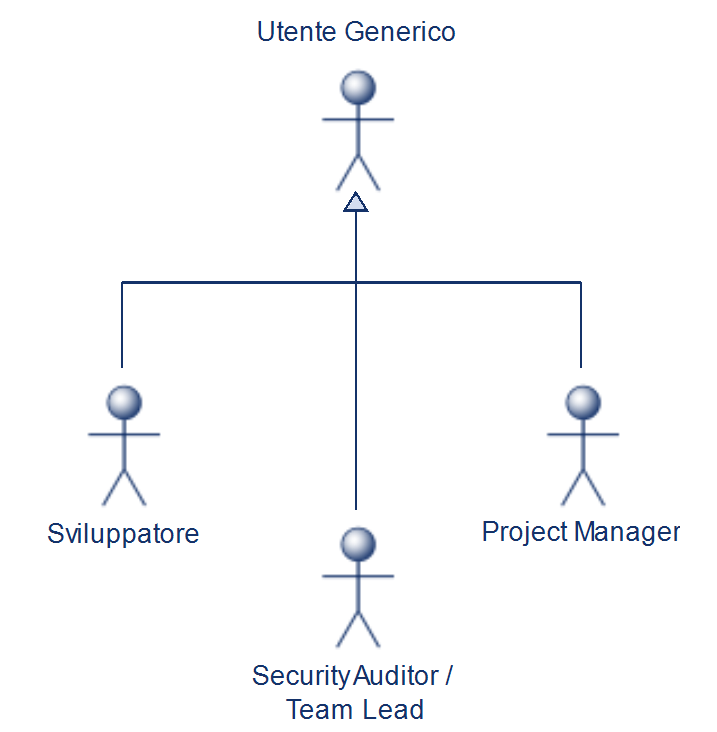
\includegraphics[width=0.6\linewidth]{ATTORI.png}
    \caption{Attori primari coinvolti}
    \label{fig:Attori}
\end{figure}

\subsubsection{\textit{Attori} Secondari}

\begin{itemize}
    \item \textbf{\textit{Repository Git}:} Il sistema di controllo di versione esterno (\textit{\glo{GitHub}{github}}). Rappresenta sia la fonte dei dati su cui gli agenti effettuano le analisi, sia la destinazione delle proposte di modifica tramite \textit{Pull Request} o \textit{\glo{Patch}{patch}}.
    
    \item \textbf{\textit{API \glo{Claude Code}{claude-code}} / Modello AI (\textit{LLM}):} I servizi di intelligenza artificiale di grandi dimensioni (\textit{LLM}) interrogati dagli agenti per individuare vulnerabilità complesse, generare codice correttivo e produrre documentazione tecnica descrittiva.
    
    \item \textbf{Sistema di Task Management:} La piattaforma esterna di tracciamento delle attività. Viene interrogata dall'Agente \textit{Changelog} per recuperare i metadati, le descrizioni e i criteri di accettazione dei \textit{\glo{Ticket}{ticket}} completati durante uno \textit{Sprint}.
    
\end{itemize}



\newpage
\subsection{\textit{Casi d'Uso} trasversali}
Di seguito sono riportati i \textit{Casi d'Uso} trasversali, ovvero validi per due o più agenti, mentre quelli specifici verranno esposti nelle sotto-sezioni apposite all'interno di ciascuna sezione dedicata a ciascun agente.

\begin{figure}[htbp]
    \centering
    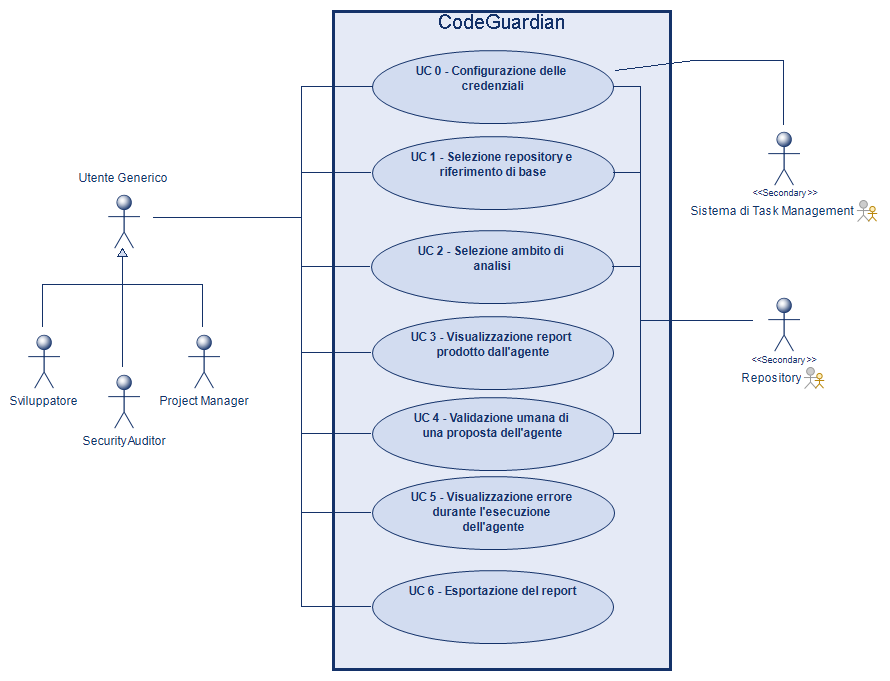
\includegraphics[width=1\linewidth]{UC trasversali.png}
    \caption{Use Cases trasversali a tutti gli Agenti}
    \label{fig:UCtrasv}
\end{figure}


\subsubsection{UC 0: Configurazione delle credenziali}\label{uc:0}
Questo caso d'uso descrive il processo attraverso il quale l'utente fornisce al sistema le credenziali necessarie per autorizzare l'accesso ai servizi esterni (come il \textit{Repository Git} e il Sistema di Task Management).

\begin{itemize}
    \item \textbf{Attore Primario}: Utente Generico.
    \item \textbf{Attori Secondari}: \textit{Repository Git}, Sistema di Task Management.
    \item \textbf{Trigger}: L'utente accede per la prima volta al sistema o necessita di aggiornare un token scaduto.
    \item \textbf{Precondizioni}:
    \begin{itemize}
        \item Il sistema è attivo e accessibile.
    \end{itemize}
    \item \textbf{Postcondizioni}: I token di accesso sono memorizzati in modo sicuro nel sistema e gli agenti sono pronti all'esecuzione.
    \item \textbf{Scenario Principale}:
        \begin{enumerate}
            \item L'utente accede alla sezione di configurazione del sistema.
            \item Il sistema richiede l'inserimento dei parametri di autenticazione.
            \item L'utente inserisce i dati richiesti.
            \item Il sistema convalida la correttezza formale e effettua una chiamata di test per verificare i permessi delle chiavi inserite.
            \item Il sistema salva le credenziali e notifica all'utente il successo dell'operazione.
        \end{enumerate}
    \item \textbf{Scenari alternativi}: 
    \begin{itemize}
        \item Al passo 4, se la chiamata di test fallisce, il sistema mostra un messaggio di errore all'utente chiedendo di reinserire le credenziali.
    \end{itemize}
\end{itemize}


\subsubsection{UC 1: Selezione \textit{repository} e riferimento di base}\label{uc:1}
Questo caso d'uso consente all'utente di indicare il repository Git e il riferimento di base su cui potranno essere eseguite le successive operazioni degli agenti. La selezione del repository non implica necessariamente l'analisi dell'intero contenuto del repository, ma definisce il contesto iniziale da utilizzare nelle funzionalità successive. È una fase preliminare comune alle funzionalità di analisi, documentazione, sicurezza e generazione di report.

\begin{itemize}
    \item \textbf{Attore Primario}: Utente Generico.
    \item \textbf{Attori Secondari}: \textit{repository} Git.
    \item \textbf{Trigger}: L'utente vuole selezionare un \textit{repository} e un riferimento specifico da utilizzare come contesto per gli agenti disponibili.
    \item \textbf{Precondizioni}:
    \begin{itemize}
        \item Il sistema è attivo e accessibile.
        \item Il \textit{repository} Git esiste ed è raggiungibile.
        \item L'utente dispone dei permessi necessari per accedere al \textit{repository}.
        \item Il repository selezionato contiene codice sorgente scritto nei linguaggi supportati dal sistema.
    \end{itemize}
    \item \textbf{Postcondizioni}: Il \textit{repository} e il riferimento selezionati sono disponibili come contesto per le funzionalità degli agenti.
    \item \textbf{Scenario Principale}:
        \begin{enumerate}
            \item L'utente accede alla sezione dedicata alla selezione del \textit{repository}.
            \item L'utente fornisce l'\textit{URL} del \textit{repository} Git.
            \item Il sistema verifica che il \textit{repository} sia raggiungibile e accessibile.
            \item L'utente seleziona il riferimento di base da utilizzare, scegliendo tra branch, \textit{\glo{Commit}{commit}} o \textit{Pull Request}.
            \item Se l'utente seleziona un branch senza indicare un \textit{Commit} specifico, il sistema considera di default l'ultimo \textit{Commit} disponibile sul branch selezionato.
            \item Il sistema registra il \textit{repository} e il riferimento selezionati come contesto per le successive operazioni degli agenti.
        \end{enumerate}
    \item \textbf{Scenari alternativi}: 
    \begin{itemize}
        \item Se l'\textit{URL} del \textit{repository} non è valido, il sistema mostra un messaggio di errore esplicativo.
        \item Se il \textit{repository} non è raggiungibile o l'utente non dispone dei permessi necessari, il sistema mostra un messaggio di errore esplicativo.
        \item Se il branch, il \textit{Commit} o la \textit{Pull Request} selezionati non esistono, il sistema mostra un messaggio di errore esplicativo.
        \item Se il repository contiene un linguaggio non supportato, il sistema avvisa l'utente che le funzionalità di analisi potrebbero non essere disponibili o generare errori.
    \end{itemize}
\end{itemize}


\subsubsection{UC 2: Selezione ambito di analisi}\label{uc:2}
Questo caso d'uso consente all'utente di delimitare la porzione del repository su cui eseguire l'analisi di un agente. L'ambito può essere ristretto a uno o più file o directory. L'analisi dell'intero repository è considerata una possibilità aggiuntiva solo se supportata dalla configurazione del sistema.

\begin{itemize}
    \item \textbf{Attore Primario}: Untente Generico.

    \item \textbf{Attori Secondari}: Repository Git.

    \item \textbf{Trigger}: L'utente vuole delimitare la parte del repository da sottoporre all'analisi di un agente.

    \item \textbf{Precondizioni}:
    \begin{itemize}
        \item È stato selezionato un repository e un riferimento di base (UC 1).
        \item Il sistema può accedere al contenuto del repository selezionato.
    \end{itemize}
    
    \item \textbf{Postcondizioni}: L'ambito di analisi selezionato è disponibile come input per l'agente interessato.

    \item \textbf{Scenario Principale}:
    \begin{enumerate}
        \item L'utente seleziona l'ambito dell'analisi, indicando o l'intero \textit{Repository} o porzioni minori (singoli file o directory).
        \item Il sistema verifica che gli elementi indicati esistano e siano accessibili.
        \item Il sistema registra l'ambito selezionato come input per l'esecuzione dell'agente interessato.
    \end{enumerate}

    \item \textbf{Scenari alternativi}:
    \begin{itemize}
        \item Se l'utente non seleziona alcun ambito, il sistema mostra un messaggio informativo e richiede di completare la selezione.
        \item Se uno o più elementi selezionati non esistono o non sono accessibili, il sistema mostra un messaggio di errore esplicativo.
        \item (desiderabile) Se l'ambito selezionato supera la capacità di elaborazione del modello, il sistema mostra un messaggio di errore esplicativo e richiede di restringere la selezione.
    \end{itemize}
\end{itemize}

\subsubsection{UC 3: Visualizzazione report prodotto dall'agente}\label{uc:3}
L'utente vuole consultare il risultato prodotto da un agente a seguito di un’analisi. Il sistema rende disponibili i report generati, permettendo all'utente di visualizzare le informazioni principali relative all’esecuzione, come criticità rilevate, suggerimenti proposti e file coinvolti.

\begin{itemize}
    \item \textbf{\textit{Attore} Primario}: Utente Generico.
    \item \textbf{Trigger}: L'utente vuole consultare l'esito dell'analisi svolta da un agente.
    \item \textbf{Precondizioni}: \begin{itemize}
    \item L'\textbf{Orchestratore} ha eseguito almeno un agente ed è disponibile almeno un report prodotto dall'agente.
    \end{itemize}
    \item \textbf{Postcondizioni}: L'utente visualizza il report generato.
    \item \textbf{Scenario Principale}:
        \begin{enumerate}
            \item L'utente accede alla sezione dedicata ai risultati dell'analisi.
            \item Il sistema mostra la lista dei report disponibili.
            \item L'utente seleziona il report desiderato.
            \item Il sistema visualizza il contenuto del report, includendo eventuali criticità, suggerimenti e file coinvolti.
        \end{enumerate}
    \item \textbf{Scenari alternativi:} \begin{itemize}
        \item Se non sono presenti report, il sistema mostra un messaggio informativo.
    \end{itemize}
\end{itemize}

\subsubsection{UC 4: Validazione umana di una proposta dell'agente}\label{uc:4}
Il sistema adotta un approccio \textit{Human-in-the-loop}, in modo che le proposte generate dagli agenti siano validate da un utente prima di essere applicate.

\begin{itemize}
    \item \textbf{\textit{Attore} Primario}: Utente Generico.
    \item \textbf{\textit{Attori} Secondari}: \textit{Repository} \textit{Git}.
    \item \textbf{Trigger}: L'utente riceve una proposta generata da un agente.
    \item \textbf{Precondizioni}: \begin{itemize}
    \item Un agente ha prodotto una proposta di modifica. La proposta è disponibile sotto forma di \textit{Pull Request}, frammento di codice o suggerimento testuale.
    \end{itemize}
    \item \textbf{Postcondizioni}: La proposta è stata accettata, modificata o rifiutata dall'utente.
    \item \textbf{Scenario Principale}:
        \begin{enumerate}
            \item L'utente apre la proposta generata dall'agente.
            \item L'utente analizza il contenuto della proposta.
            \item L'utente decide se accettare, modificare o rifiutare la proposta.
            \item Il sistema registra l'esito della validazione.
        \end{enumerate}
\end{itemize}

\subsubsection{UC 5: Visualizzazione errore durante l’esecuzione dell’agente}\label{uc:5}
Durante l’esecuzione di un agente può verificarsi un errore che impedisce il completamento dell’analisi o la generazione dell’output richiesto. In questo caso il sistema mostra all'utente un messaggio esplicativo, indicando la causa dell’errore e, quando possibile, una possibile azione correttiva.

\begin{itemize}
    \item \textbf{\textit{Attore} Primario}: Utente Generico.
    \item \textbf{Trigger}: L'esecuzione di un agente termina con errore.
    \item \textbf{Precondizioni}: \begin{itemize}
    \item È stata avviata l'esecuzione di un agente. Si verifica un errore durante l'analisi o la generazione dell'output.
    \end{itemize}
    \item \textbf{Postcondizioni}: L'utente visualizza un messaggio di errore esplicativo.
    \item \textbf{Scenario Principale}:
        \begin{enumerate}
            \item L'agente incontra un errore durante l'esecuzione.
            \item L'\textbf{Orchestratore} riceve l'esito negativo.
            \item Il sistema mostra all'utente un messaggio che descrive la causa dell'errore (es. timeout di risposta dal modello \textit{AI}, formato di output dell'\textit{LLM} non interpretabile, file di configurazione assente, formato del report non generabile, superamento del limite massimo di file/righe di codice elaborabili, superamento delle quote di utilizzo API).
            \item Il sistema indica, se possibile, un'azione correttiva.
        \end{enumerate}
\end{itemize}

\subsubsection{UC 6: Esportazione del report}\label{uc:6}
L'utente vuole esportare un report generato da un agente per conservarlo, 
condividerlo o utilizzarlo nelle successive attività di sviluppo e verifica. Il sistema permette di selezionare il report desiderato e di salvarlo in uno dei formati disponibili.

\begin{itemize}
    \item \textbf{\textit{Attore} Primario}: Utente Generico.
    \item \textbf{Trigger}: L'utente vuole esportare e salvare il risultato di un'analisi di un agente in uno dei formati disponibili.
    \item \textbf{Precondizioni}: \begin{itemize}
    \item È disponibile almeno un report generato da un agente.
    \end{itemize}
    \item \textbf{Postcondizioni}: Il report è stato esportato nel formato scelto.
    \item \textbf{Scenario Principale}:
        \begin{enumerate}
            \item L'utente seleziona un report.
            \item L'utente sceglie il formato di esportazione.
            \item Il sistema genera il file esportabile.
            \item L'utente scarica o salva il report.
        \end{enumerate}
    \item \textbf{Scenari alternativi:} \begin{itemize}
    \item Se l'esportazione fallisce, il sistema mostra un messaggio di errore.
    \end{itemize}
\end{itemize}


\newpage
\section{Agente Docs: Documentazione e \textit{README}}

\subsection{Introduzione all'agente}
L'Agente di Documentazione e \textit{README} rappresenta un pilastro fondamentale per la qualità del lavoro quotidiano degli sviluppatori e per la stabilità del progetto Code Guardian. Sappiamo bene come, nei cicli di sviluppo veloci, la documentazione sia spesso la prima a perdere il passo rispetto al codice, diventando presto superata. Questo agente nasce proprio per risolvere tale problema: il suo compito è automatizzare tutto il processo di aggiornamento. In questo modo, garantiamo che il file \texttt{\textit{README}.md} e l'intera documentazione tecnica, sia quella interna al codice che quella dedicata alle \textit{API}, siano sempre uno specchio fedele e puntuale dell'evoluzione del progetto, in qualsiasi momento.

\subsection{Obiettivi e Funzionalità}
L'agente si focalizza su tre aree critiche:

\begin{enumerate}

    \item \textbf{Manutenzione del \textit{README}}: Automazione della creazione e dell'aggiornamento del file principale di presentazione del \textit{Repository}, adattandolo dinamicamente alle evoluzioni della piattaforma.

    \item \textbf{Gestione della documentazione inline}: Analisi semantica del codice per la generazione di \textit{Docstring} e \textit{JSDoc}, assicurando che ogni modulo sia correttamente commentato.

    \item \textbf{Documentazione delle \textit{API}}: Estrazione automatizzata degli \textit{\glo{Endpoint}{endpoint}} per la creazione di guide tecniche per gli utilizzatori del servizio.

\end{enumerate}

\newpage
\subsection{\textit{Casi d'Uso}}
Di seguito i \textit{Casi d'Uso} dell'Agente Docs.

\begin{figure}[htbp]
    \centering
    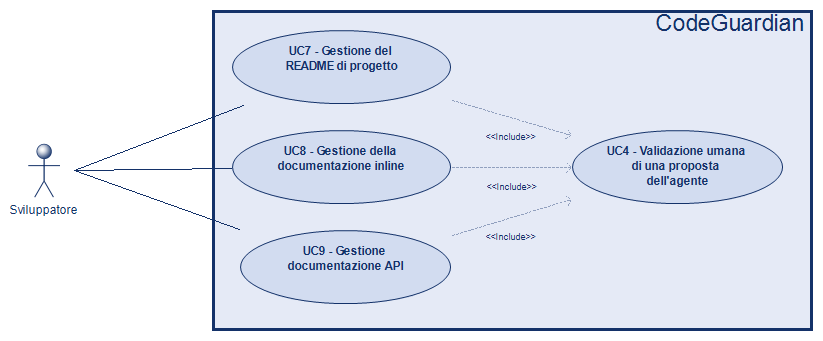
\includegraphics[width=1\linewidth]{UC Docs.png}
    \caption{Use Cases dell'Agente Docs}
    \label{fig:UCDocs}
\end{figure}

\subsubsection{UC 7: Gestione del \textit{README} di Progetto}\label{uc:7}
Questo è il \textit{Caso d'Uso} generico per la gestione automatizzata del \texttt{\textit{README}.md} del Progetto.

\begin{itemize}
    \item \textbf{\textit{Attore} Primario}: Sviluppatore.
    \item \textbf{\textit{Attori} Secondari}: \textit{Repository} \textit{Git}.
    \item \textbf{Trigger}: Lo Sviluppatore richiede l'intervento tramite l'\textbf{Orchestratore}.
    \item \textbf{Precondizioni}: 
        \begin{itemize}
            \item È stato selezionato un \textit{repository} e un riferimento di base (UC 1).
            \item (Opzionale) Esiste un modello personalizzato per il \textit{README}.
        \end{itemize}
    \item \textbf{Postcondizioni}: È disponibile una proposta di creazione o aggiornamento del \texttt{\textit{README}.md}, pronta per la validazione umana, o il \texttt{\textit{README}.md} è già aggiornato.
    \item \textbf{Scenario Principale}:
        \begin{enumerate}
            \item L'\textbf{Orchestratore} notifica l'Agente Docs della necessità di gestire il \textit{README}.
            \item L'Agente analizza file di configurazione e struttura delle cartelle.
            \item L'Agente crea o aggiorna il \textit{README} secondo il modello personalizzato, se disponibile, o quello di default.
            \item L'Agente propone il prodotto tramite \textit{Pull Request}.
        \end{enumerate}
    \item \textbf{Scenario alternativo}:
        \begin{itemize}
            \item L'analisi non rileva cambiamenti: non vengono generate proposte di aggiornamento, lo Sviluppatore viene informato e lo UC termina.
            \item L'Agente non riceve risposta dall'\textit{LLM} entro il tempo limite oppure riceve un output la cui struttura non è parsabile dal sistema, l'elaborazione viene interrotta e il flusso passa all'UC 5 per la visualizzazione dell'errore.
        \end{itemize}
    \item \textbf{Inclusioni}: UC 4 - Validazione umana di una proposta dell’agente.
\end{itemize}

\subsubsection{UC 8: Gestione della Documentazione Inline (\textit{Docstring}/\textit{JSDoc})}\label{uc:8}
L'agente interviene nel codice sorgente per garantire che ogni componente sia documentato correttamente.

\begin{itemize}
    \item \textbf{\textit{Attore} Primario}: Sviluppatore.
    \item \textbf{Trigger}: Richiesta esplicita da parte dello Sviluppatore verso l'\textbf{Orchestratore}.
    \item \textbf{Precondizioni}:  
        \begin{itemize}
            \item È stato selezionato un ambito di analisi (UC 2).
        \end{itemize}
    \item \textbf{Postcondizioni}: Lo Sviluppatore dispone di una proposta di documentazione inline da validare o la documentazione è già aggiornata.
    \item \textbf{Scenario Principale}:
        \begin{enumerate}
            \item L'Agente individua funzioni o classi prive di documentazione, con documentazione obsoleta o non conforme.
            \item L'Agente interpreta la logica della funzione, i parametri di input e il valore di ritorno o lo scopo e le caratteristiche della classe.
            \item Per ogni classe/funzione individuata, l'Agente genera una proposta di commento standardizzato (\textit{JSDoc}).
            \item Il sistema rende le proposte disponibili per validazione allo Sviluppatore.
        \end{enumerate}
    \item \textbf{Scenario alternativo}:
    \begin{itemize}
        \item Se l'Agente non riesce a interpretare una classe/funzione, invece di una proposta viene generato un avvertimento per quella specifica classe/funzione e l'analisi passa a quella seguente, se presente.
        \item Se le modifiche al codice non richiedono di cambiare la documentazione, non vengono generate proposte di aggiornamento, lo Sviluppatore viene informato e l'UC termina.
        \item Se l'Agente non riceve risposta dall'\textit{LLM} entro il tempo limite oppure riceve un output la cui struttura non è parsabile dal sistema, l'elaborazione viene interrotta e il flusso passa all'UC 5 per la visualizzazione dell'errore.
    \end{itemize}
    \item \textbf{Inclusioni}:\begin{itemize}
    \item UC 4: Validazione umana di una proposta dell’agente.
    \end{itemize}
\end{itemize}

\subsubsection{UC 9: Gestione Documentazione \textit{API}}\label{uc:9}
L'agente estrae le definizioni degli \textit{Endpoint} per creare una guida tecnica per i consumatori delle \textit{API}.

\begin{itemize}
    \item \textbf{\textit{Attore} Primario}: Sviluppatore.
    \item \textbf{Trigger}: Richiesta esplicita di generazione prima di un rilascio.
    \item \textbf{Precondizioni}: \begin{itemize}
    \item È stato selezionato un ambito di analisi (UC 2).
    \end{itemize}
    \item \textbf{Postcondizioni}: È disponibile una proposta di documento tecnico (\texttt{\textit{API}.md}) o il documento è già aggiornato.
    \item \textbf{Scenario Principale}:
        \begin{enumerate}
            \item L'Agente scansiona i file dei controller e i file delle \textit{\glo{Rotte}{rotte}}.
            \item Estrazione di: metodo HTTP, URL, header, \textit{\glo{Payload}{payload}} richiesto e risposte possibili.
            \item Formattazione delle informazioni nel file \texttt{\textit{API}.md} in formato \textit{\glo{Markdown}{markdown}}.
            \item Il Sistema mette a disposizione la proposta di documento allo Sviluppatore per la validazione.
        \end{enumerate}
    \item \textbf{Scenario alternativo}:
    \begin{itemize}
        \item Se l'analisi non rileva cambiamenti, non vengono generate proposte di aggiornamento, lo Sviluppatore è informato e l'UC termina.
        \item Se l'Agente non riceve risposta dall'\textit{LLM} entro il tempo limite oppure riceve un output la cui struttura non è parsabile dal sistema, l'elaborazione viene interrotta e il flusso passa all'UC 5 per la visualizzazione dell'errore.
    \end{itemize}
    \item \textbf{Inclusioni}: \begin{itemize}
    \item UC 4: Validazione umana di una proposta dell’agente.
    \end{itemize}
\end{itemize}

\newpage
\section{Agente OWASP: Scansione \textit{Vulnerabilità} \textit{OWASP}}

\subsection{Introduzione all'agente}
L'Agente di Scansione Vulnerabilità \textit{OWASP} ha l'obiettivo di supportare il \textit{Security Auditor} nell'individuazione di possibili \textit{Vulnerabilità} di sicurezza presenti nel codice sorgente del \textit{Repository}. L'analisi di sicurezza viene svolta facendo riferimento alle principali categorie di rischio definite da \textit{OWASP} individuabili tramite analisi del codice, come: \textit{\glo{Injection}{injection}}, gestione non sicura dell'autenticazione, controllo degli accessi incompleto, gestione errata di dati sensibili, configurazioni insicure, ecc.
\\ 
L'agente non garantisce la copertura esaustiva dell'intera \textit{OWASP} Top 10. Il suo scopo è fornire una revisione automatizzata assistita, producendo segnalazioni, priorità e suggerimenti di \textit{\glo{Remediation}{remediation}} che devono essere successivamente valutati da un \textit{Team Lead} o \textit{Security Auditor}.

\subsection{Obiettivi e Funzionalità}
L'agente si concentra su tre aree principali:
\begin{enumerate}
\item \textbf{Analisi delle \textit{Vulnerabilità} \textit{OWASP}}: individuazione di pattern di codice potenzialmente riconducibili a \textit{Vulnerabilità} note, come SQL \textit{Injection}, uso insicuro di funzioni crittografiche, esposizione di informazioni sensibili, \textit{\glo{Hardcoded secrets}{hardcoded-secrets}}, ecc.
\item \textbf{Verifica delle policy interne di sicurezza}: controllo dell'aderenza del codice alle regole definite dal team nel file CLAUDE.md, secondo un approccio di tipo \textit{Policy-as-code}.
\item \textbf{Generazione di remediation}: produzione di suggerimenti testuali o modifiche al codice correttive per mitigare le vulnerabilità o le non conformità rilevate, senza applicare modifiche automatiche prima della validazione umana.
\end{enumerate}

\newpage
\subsection{\textit{Casi d'Uso}}
Di seguito i \textit{Casi d'Uso} dell'Agente OWASP.

\subsubsection{UC 10: Esecuzione Scansione \textit{Vulnerabilità} (\textit{OWASP})}\label{uc:10}
L'agente utilizza le \textit{API} di \textit{Claude Code} per identificare \textit{Vulnerabilità} standard di sicurezza nel codice sorgente.

\begin{figure}[htbp]
    \centering
    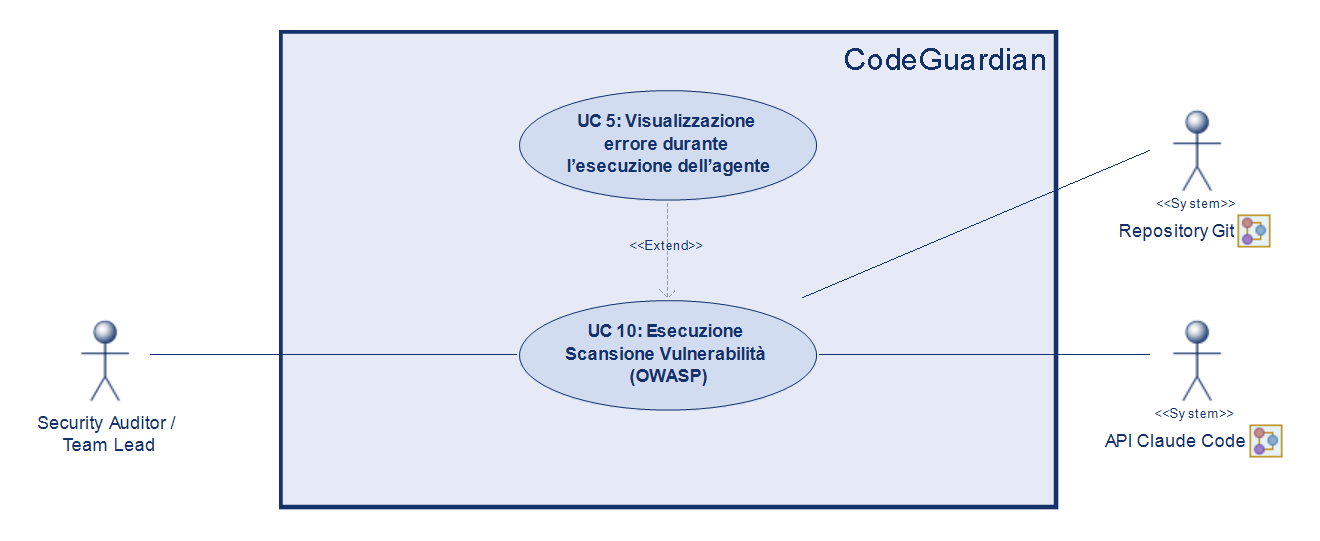
\includegraphics[width=1\linewidth]{UML UC10.png}
    \caption{Use Case Scansione Vulnerabilità}
    \label{fig:UC10}
\end{figure}

\begin{itemize}
\item
  \textbf{\textit{Attore} Primario}: \textit{Security Auditor} / \textit{Team Lead}.
\item
  \textbf{\textit{Attori} Secondari}: \textit{Repository} \textit{Git}, \textit{API} \textit{Claude Code}.
\item
  \textbf{Trigger}: Il \textit{Security Auditor} richiede una scansione di sicurezza per identificare \textit{Vulnerabilità}.
\item
  \textbf{Precondizioni}:
  \begin{itemize}
  \item È stato selezionato un ambito di analisi (UC 2).
  \item
    L'Agente OWASP è correttamente configurato con le \textit{API} Key di \textit{Claude Code}.
\end{itemize}
\item
    \textbf{Postcondizioni}: Viene generato un report tecnico delle \textit{Vulnerabilità} rilevate. Ogni \textit{Vulnerabilità} rilevata è descritta con categoria, gravità e riferimento al codice interessato.
\item
  \textbf{Scenario Principale}:

  \begin{enumerate}
  \item 
  L'Agente OWASP riceve dall'\textbf{Orchestratore} il codice sorgente relativo all'ambito di analisi selezionato.
  \item
    L'Agente OWASP interroga le \textit{API} di \textit{Claude Code} inviando il codice per l'analisi.
\item
    L'Agente OWASP analizza il codice cercando pattern
    riconducibili alle \textit{Vulnerabilità} della Top 10 \textit{OWASP} (es. SQL
    \textit{Injection}, \textit{\glo{XSS}{xss}}, \textit{Hardcoded secrets}).
\item
    L'Agente OWASP riceve l'esito dell'analisi.
\item
    L'Agente OWASP associa ogni \textit{Vulnerabilità} al file e, se disponibile, alla porzione di codice interessata.
\item
    L'Agente OWASP classifica ogni \textit{Vulnerabilità} trovata nelle categorie di Top 10 \textit{OWASP}.
\item
    L'Agente OWASP formatta i risultati evidenziando la
    gravità (High, Medium, Low) di ogni falla trovata.
\item
    L'Agente OWASP inserisce le \textit{Vulnerabilità}, la loro classificazione e le gravità nel report finale.
\end{enumerate}

\item \textbf{Scenario Alternativo}: 
\begin{itemize}
    \item Se non vengono rilevate \textit{Vulnerabilità}, l’Agente genera un report che indica l’assenza di criticità individuate.
    \item L'Agente non riceve risposta dall'\textit{LLM} entro il tempo limite oppure riceve un output la cui struttura non è parsabile dal sistema, l'elaborazione viene interrotta e il flusso passa all'UC 5 per la visualizzazione dell'errore.
\end{itemize}
\end{itemize}


\subsubsection{UC 11: Verifica Conformità "\textit{Policy-as-code}" (CLAUDE.md)}\label{uc:11}
L'agente verifica che il codice rispetti le regole
specifiche definite dal team nel file di configurazione.

\begin{figure}[htbp]
    \centering
    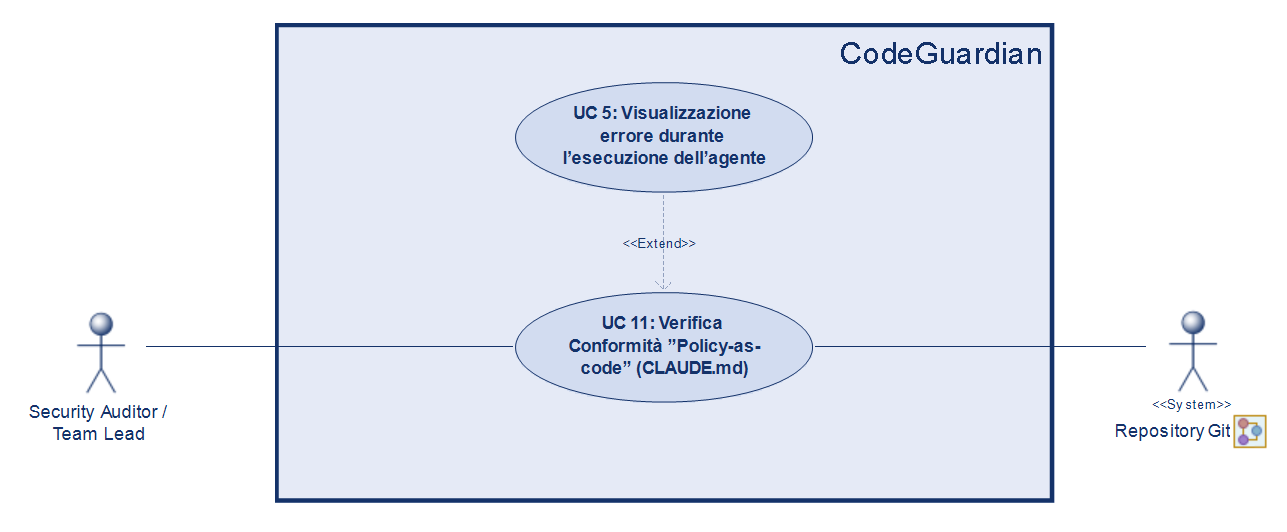
\includegraphics[width=1\linewidth]{UML UC11.png}
    \caption{Use Case Conformità ”Policy-as-code”}
    \label{fig:UC11}
\end{figure}

\begin{itemize}
\item
  \textbf{\textit{Attore} Primario}: \textit{Security Auditor} / \textit{Team Lead}.
\item
  \textbf{\textit{Attori} Secondari}: \textit{Repository Git}.
\item
  \textbf{Trigger}: Il \textit{Security Auditor} richiede una revisione di conformità.
\item \textbf{Precondizioni}:
\begin{itemize}
    \item È stato selezionato un ambito di analisi (UC 2).
    \item Il codice sorgente è accessibile.
\end{itemize}
\item
  \textbf{Postcondizioni}: Viene prodotto un elenco di non-conformità rispetto alle policy di progetto.
\item
  \textbf{Scenario Principale}:
  
  \begin{enumerate}
  \item 
  L'Agente verifica che il file CLAUDE.md sia presente, leggibile e interpretabile.
  \item
    L'Agente OWASP legge il contenuto del file CLAUDE.md per
    estrarre il contesto e le regole (es. "usa sempre questa libreria
    per il logging", "non usare variabili globali").
\item
    L'Agente analizza il codice sorgente confrontandolo
    con le direttive estratte.
\item
    L'Agente identifica eventuali deviazioni dalle
    pratiche concordate dal team.
\item
    L'Agente genera un elenco di violazioni della policy
    interna.
\end{enumerate}
\item
  \textbf{Scenari alternativi}:
  \textbf{Scenari alternativi}:
\begin{itemize}
    \item \textbf{Il file CLAUDE.md non è presente}: il sistema rileva l'assenza del file, interrompe la verifica delle policy interne e delega la gestione del fallimento all'UC 5 per mostrare il messaggio d'errore specifico.
    \item \textbf{Il file CLAUDE.md non è leggibile o non contiene regole interpretabili}: il sistema rileva l'impossibilità di analizzare il file, interrompe la verifica delle policy interne e delega la gestione del fallimento all'UC 5 per mostrare il messaggio d'errore specifico.
    \item \textbf{Il file CLAUDE.md contiene regole in palese contraddizione logica}: l'Agente OWASP legge il contenuto del file per estrarre le regole, rileva un conflitto logico insormontabile tra due o più direttive, quindi interrompe la verifica delle policy interne e delega la gestione del fallimento all'UC 5.
\end{itemize}
    \end{itemize}

\newpage
\subsubsection{UC 12: Generazione Suggerimenti di \textit{Remediation}}\label{uc:12}
L'agente fornisce soluzioni pratiche per correggere i
problemi di sicurezza o le violazioni di policy trovate.

\begin{figure}[htbp]
    \centering
    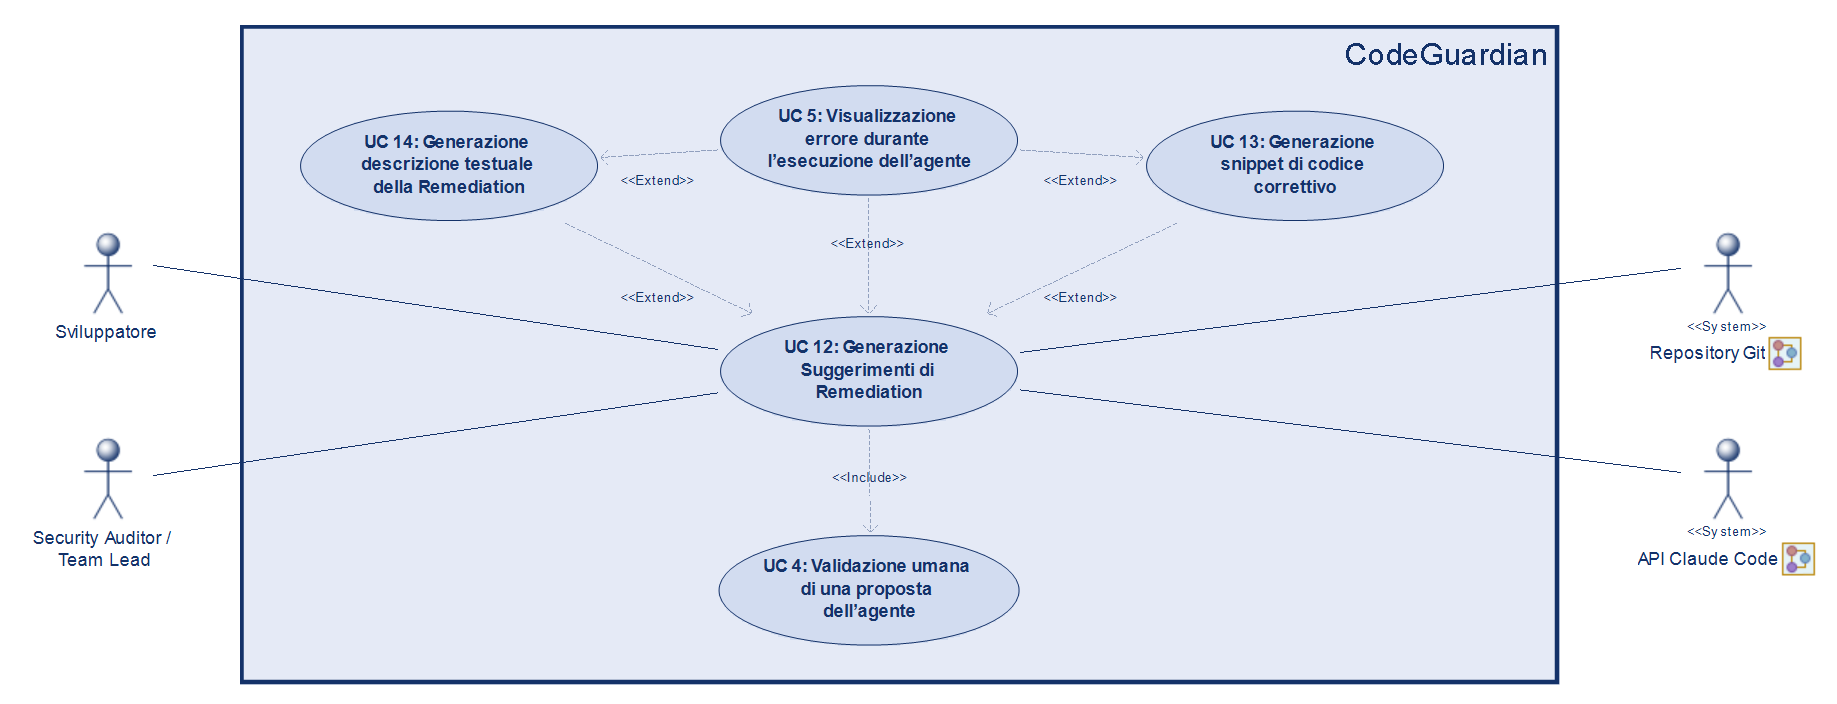
\includegraphics[width=1\linewidth]{UML UC12,13,14.png}
    \caption{Use Cases Generazione Suggerimenti di Remediation}
    \label{fig:UC12,13,14}
\end{figure}

\begin{itemize}
\item
  \textbf{\textit{Attore} Primario}: \textit{Security Auditor} / \textit{Team Lead} / Sviluppatore.
\item
  \textbf{\textit{Attori} Secondari}: \textit{Repository} Git, \textit{API} \textit{Claude Code}.
\item
  \textbf{Trigger}: Conclusione con esito positivo (rilevamento falle) degli UC 10 o UC 11 e richiesta del utente di generare suggerimenti di \textit{Remediation}.
\item
  \textbf{Precondizioni}: \begin{itemize}
  \item Sono state identificate \textit{Vulnerabilità} o violazioni di policy.
  \end{itemize}
\item
  \textbf{Postcondizioni}: Il \textit{Security Auditor} riceve indicazioni chiare su come
  correggere il codice per renderlo conforme.
\item
  \textbf{Scenario Principale}:

  \begin{enumerate}
  \def\labelenumi{\arabic{enumi}.}
    \item 
    Per ogni vulnerabilità o violazione rilevata, l'Agente analizza il contesto e la porzione di codice interessata.
    \item 
    L'Agente determina il livello di localizzazione possibile per la risoluzione del problema.
    \item 
    Il flusso si estende per generare uno snippet di codice correttivo (UC 13) oppure una descrizione testuale (UC 14).
    \item
    Il \textit{Security Auditor} consulta vulnerabilità, gravità, file coinvolto, spiegazione e proposta correttiva.
    \end{enumerate}
\item \textbf{Scenario Alternativo}: 
\begin{itemize}
    \item L'Agente non riceve risposta dall'\textit{LLM} entro il tempo limite oppure riceve un output la cui struttura non è parsabile dal sistema, l'elaborazione viene interrotta e il flusso passa all'UC 5 per la visualizzazione dell'errore.
\end{itemize}
    
\item 
  \textbf{Inclusioni}:
    \begin{itemize}
        \item UC 4: Validazione umana di una proposta dell'agente.
    \end{itemize}    
\item 
  \textbf{Estensioni}: 
    \begin{itemize}
        \item UC 13: Generazione snippet di codice correttivo.
        \item UC 14: Generazione descrizione testuale della remediation.
    \end{itemize}
\end{itemize}

\subsubsection{UC 13: Generazione snippet di codice correttivo}\label{uc:13}
Descrive la generazione di un frammento di codice alternativo per correggere una \textit{Vulnerabilità} o una non conformità.

\begin{itemize}
    \item \textbf{\textit{Attore} Primario}: \textit{Security Auditor} / \textit{Team Lead} / Sviluppatore.
    \item \textbf{\textit{Attori} Secondari}: \textit{Repository} Git, \textit{API} \textit{Claude Code}.
    \item \textbf{Trigger}: Una \textit{Vulnerabilità} o non conformità può essere corretta tramite una modifica puntuale al codice.
    \item \textbf{Precondizioni}:
        \begin{itemize}
            \item La \textit{Vulnerabilità} è sufficientemente circoscritta nel codice.
            \item L’Agente OWASP può proporre una soluzione locale senza modifiche architetturali.
        \end{itemize}
    \item \textbf{Postcondizioni}: Il \textit{Security Auditor} visualizza uno snippet di codice correttivo da valutare manualmente.
    \item \textbf{Scenario Principale}:
        \begin{enumerate}
            \item L’Agente OWASP seleziona il frammento di codice vulnerabile.
            \item L’Agente OWASP richiede una versione corretta del frammento.
            \item Il modello genera uno snippet alternativo.
            \item L’Agente OWASP presenta al \textit{Security Auditor} il confronto tra codice originale e codice proposto.
        \end{enumerate}
    \item \textbf{Scenario Alternativo}: 
    \begin{itemize}
    \item L'Agente non riceve risposta dall'\textit{LLM} entro il tempo limite oppure riceve un output la cui struttura non è parsabile dal sistema, l'elaborazione viene interrotta e il flusso passa all'UC 5 per la visualizzazione dell'errore.
\end{itemize}
\end{itemize}

\subsubsection{UC 14: Generazione descrizione testuale della \textit{Remediation}}\label{uc:14}
Descrive la generazione di una spiegazione testuale della correzione da effettuare.

\begin{itemize}
    \item \textbf{\textit{Attore} Primario}: \textit{Security Auditor} / \textit{Team Lead} / Sviluppatore.
    \item \textbf{\textit{Attori} Secondari}: \textit{Repository} Git, \textit{API} \textit{Claude Code}.
    \item \textbf{Trigger}: Una \textit{Vulnerabilità} o non conformità non può essere risolta in modo affidabile tramite uno snippet di codice.
    \item \textbf{Precondizioni}:\begin{itemize}
        \item È disponibile una \textit{Vulnerabilità} o non conformità rilevata, l’agente dispone del contesto sufficiente per descrivere il problema.
    \end{itemize}
    \item \textbf{Postcondizioni}: Il \textit{Security Auditor} riceve una descrizione chiara della \textit{Remediation} consigliata.
    \item \textbf{Scenario Principale}:
        \begin{enumerate}
            \item L’Agente OWASP analizza il problema rilevato.
            \item L’Agente OWASP genera una spiegazione della causa del problema.
            \item L’Agente OWASP descrive le azioni consigliate per mitigare o correggere il problema.
            \item L’Agente OWASP inserisce la descrizione nel report finale.
        \end{enumerate}
    \item \textbf{Scenario Alternativo}: 
    \begin{itemize}
    \item L'Agente non riceve risposta dall'\textit{LLM} entro il tempo limite oppure riceve un output la cui struttura non è parsabile dal sistema, l'elaborazione viene interrotta e il flusso passa all'UC 5 per la visualizzazione dell'errore.
\end{itemize}
\end{itemize}

\newpage

\newpage
\section{Agente Changelog: \textit{Changelog} da \textit{User Stories}}

\subsection{Introduzione all'agente}
L'Agente di \textit{Changelog} da \textit{User Stories} funge da mediatore semantico tra il progresso puramente tecnico del team di sviluppo e le necessità informative degli \textit{Stakeholder} di business come il \textit{Project Manager}. In un contesto \textit{\glo{Agile}{agile}}, comprendere l'impatto reale di uno \textit{Sprint} può essere complesso per figure non tecniche se i resoconti si limitano a liste di \textit{Commit} o \textit{Ticket} criptici. Questo agente automatizza la traduzione delle attività concluse in report chiari, garantendo che ogni aggiornamento del software sia accompagnato da una narrazione del valore di business generato, senza però tralasciare il dettaglio tecnico necessario alla manutenzione interna.

\subsection{Obiettivi e Funzionalità}
L'agente si concentra sulla sintesi e trasformazione del progresso di progetto attraverso tre direttrici:
\begin{enumerate}
\item \textbf{Recupero e Analisi dei Dati}: Integrazione con il sistema di task management \textit{GitHub} \textit{\glo{Issues}{issue}} per l'estrazione automatizzata dei task completati.
\item \textbf{Sintesi Semantica Multitarget}: Generazione di report differenziati; uno tecnico (\textit{Changelog} Tecnico) per il team di sviluppo e uno di valore (\textit{Changelog} di Business) per i clienti e il management.
\item \textbf{Validazione e Qualità del Contesto}: Monitoraggio della qualità informativa dei task per prevenire la generazione di report ambigui o privi di valore.
\end{enumerate}

\newpage
\subsection{\textit{Casi d'Uso}}
Di seguito i \textit{Casi d'Uso} dell'Agente Changelog.

\subsubsection{UC 15: Recupero e Filtraggio \textit{User Stories}}\label{uc:15}
Questo caso d'uso riguarda l'estrazione delle attività completate dai sistemi esterni per avviare il processo di analisi.

\begin{figure}[htbp]
    \centering
    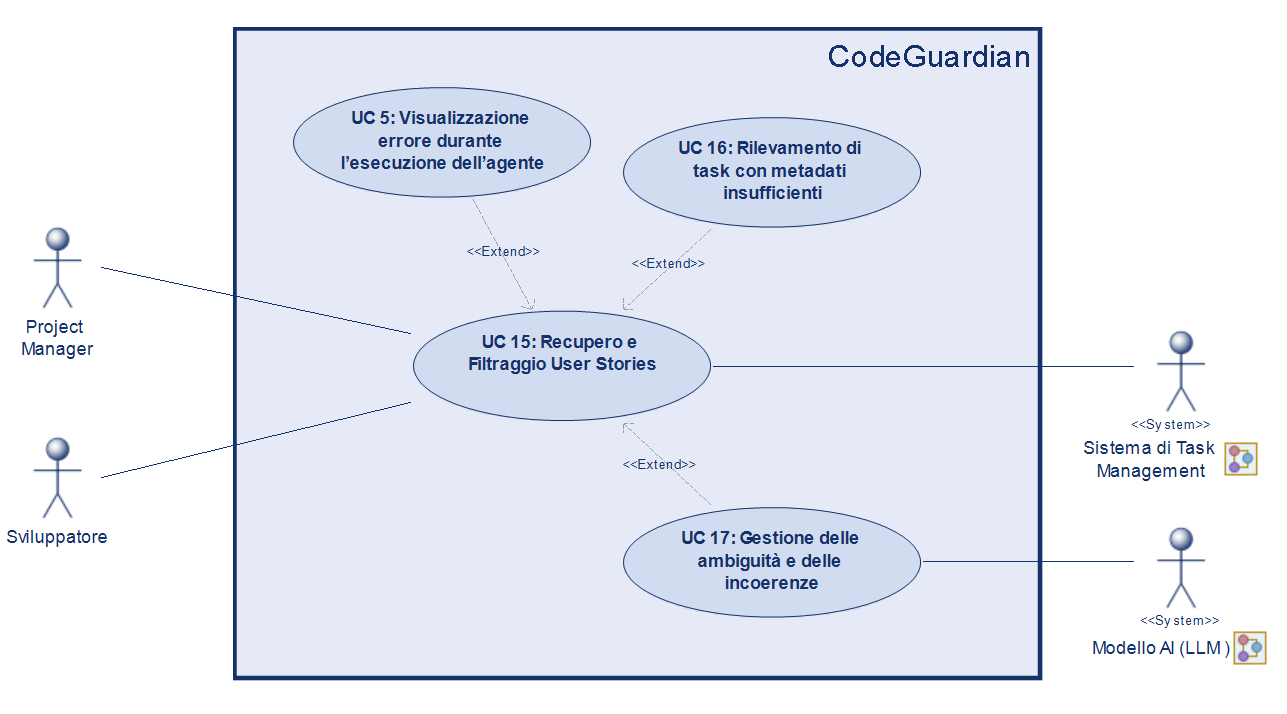
\includegraphics[width=1\linewidth]{UML UC15,16,17.png}
    \caption{Use Cases Recupero e Filtraggio User Stories}
    \label{fig:UC15,16,17}
\end{figure}

\begin{itemize}
\item \textbf{\textit{Attore} Primario}: Sviluppatore / \textit{Project Manager}.
\item \textbf{\textit{Attori} Secondari}: Sistema di Task Management \textit{GitHub Issues}.
\item \textbf{Trigger}: Lo Sviluppatore  o il \textit{Project Manager} richiede la generazione del report a conclusione di uno \textit{Sprint}.
\item \textbf{Precondizioni}:
\begin{itemize}
\item L'Agente Changelog dispone delle credenziali e dei token di accesso validi per le \textit{API} del sistema esterno.
\item È stato specificato un identificativo valido per lo \textit{Sprint} (\textit{Sprint} ID).
\item Le task completate durante lo \textit{Sprint} si trovano in uno stato terminale positivo.
\end{itemize}
\item \textbf{Postcondizioni}: L'Agente dispone delle \textit{User Stories} e dei task completati nello \textit{Sprint} selezionato.
\item \textbf{Scenario Principale}:
\begin{enumerate}
\item Il \textit{Project Manager} o lo Sviluppatore seleziona lo \textit{Sprint} da analizzare comunicando lo \textit{Sprint} ID.
\item Il sistema esterno restituisce la lista di tutte le lavorazioni associate.
\item L'Agente filtra la lista, mantenendo esclusivamente le \textit{User Stories} e i task che si trovano in uno stato terminale positivo (es. \texttt{Done}, \texttt{Closed}).
\item L'Agente estrae da ogni task i campi fondamentali: Titolo, Descrizione, Criteri di Accettazione e Commenti rilevanti.
\item L'Agente mappa i dati in una struttura interna e li memorizza temporaneamente.
\end{enumerate}
\item \textbf{Scenari alternativi}: 
    \begin{itemize}
        \item Se lo Sprint ID non esiste o non contiene task completati il sistema di Task Management restituisce un errore o una lista vuota, l'agente interrompe l'esecuzione e il flusso passa all'UC 5.
    \end{itemize}

\item 
  \textbf{Estensioni}: 
    \begin{itemize}
        \item UC 16: Rilevamento di task con metadati insufficienti e segnalazione all'utente.
\item UC 17: Gestione delle ambiguità se l'Agente Changelog rileva discrepanze tra titolo e contenuto tecnico.
    \end{itemize}

\end{itemize}

\subsubsection{UC 16: Rilevamento di task con metadati insufficienti}\label{uc:16}
\begin{itemize}
\item \textbf{\textit{Attore} Primario}: Sviluppatore / \textit{Project Manager}.
\item \textbf{\textit{Attori} Secondari}: Sistema di Task Management.
\item \textbf{Trigger}: Durante l'esecuzione del recupero (UC 15), l'agente individua una o più \textit{User Stories} prive di descrizione o di criteri di accettazione minimi.
\item \textbf{Precondizioni}: \begin{itemize}
\item L'Agente ha superato la fase di autenticazione \textit{API} e ha estratto la lista grezza delle task dello \textit{Sprint}.
\end{itemize}
\item \textbf{Postcondizioni}: Il flusso di generazione dei report (UC 18 / UC 19) prosegue solo per le task complete di tutti i metadati, mentre l'utente riceve la notifica tempestiva dei dati mancanti da integrare manualmente nei task incompleti.
\item \textbf{Scenario Principale}:
\begin{enumerate}
\item L'Agente analizza il contenuto testuale dei campi informativi di ogni task.
\item L'Agente rileva che una o più task presentano un livello informativo nullo o sotto la soglia minima stabilita dal sistema.
\item L'Agente contrassegna internamente queste task come "Non documentabili per scarsità di dati" ed esclude i relativi ID dal flusso di generazione automatica.
\item Il sistema genera un avviso nel log di esecuzione per informare l'utente delle specifiche task scartate.
\end{enumerate}
\end{itemize}

\subsubsection{UC 17: Gestione delle ambiguità e delle incoerenze}\label{uc:17}
\begin{itemize}
\item \textbf{\textit{Attore} Primario}: Sviluppatore / \textit{Project Manager}.
\item \textbf{\textit{Attori} Secondari}: Modello AI (\textit{LLM}).
\item \textbf{Trigger}: Durante la validazione dei dati aggregati nell'UC 15, l'agente rileva una forte discrepanza semantica tra il titolo/descrizione della \textit{User Story} e i dati tecnici correlati (es. log dei \textit{Commit} associati).
\item \textbf{Precondizioni}: \begin{itemize}
\item I dati della \textit{User Story} e i dati del \textit{Repository} \textit{Git} (\textit{Commit}/branch) sono stati recuperati con successo e sono pronti per l'analisi.
\end{itemize}
\item \textbf{Postcondizioni}: Viene intercettato un potenziale errore di contesto prima della generazione del report definitivo, garantendo la perfetta coerenza tra ciò che viene dichiarato nel \textit{Changelog} Tecnico e ciò che viene spiegato nel \textit{Changelog} di Business.
\item \textbf{Scenario Principal}:
\begin{enumerate}
\item L'Agente esegue un confronto semantico automatico tramite \textit{LLM} tra la documentazione della task e l'effettivo codice/messaggio di \textit{Commit} associato.
\item L'Agente identifica un conflitto (es. task registrata come "Modifica Testi" ma modifiche reali focalizzate sulla "Sicurezza delle API").
\item L'Agente contrassegna la voce come "Ambigua".
\item Il sistema presenta una notifica visiva allo Sviluppatore o al Sviluppatore / \textit{Project Manager}, richiedendo una risoluzione manuale o una conferma su quale contesto dare priorità (Documentale o Tecnico).
\end{enumerate}
\end{itemize}

\newpage
\subsubsection{UC 18: Generazione \textit{Changelog} Tecnico (Dev-to-Dev)}\label{uc:18}
L'Agente genera un Changelog Dev-to-Dev partendo dai dati delle User Stories.

\begin{figure}[htbp]
    \centering
    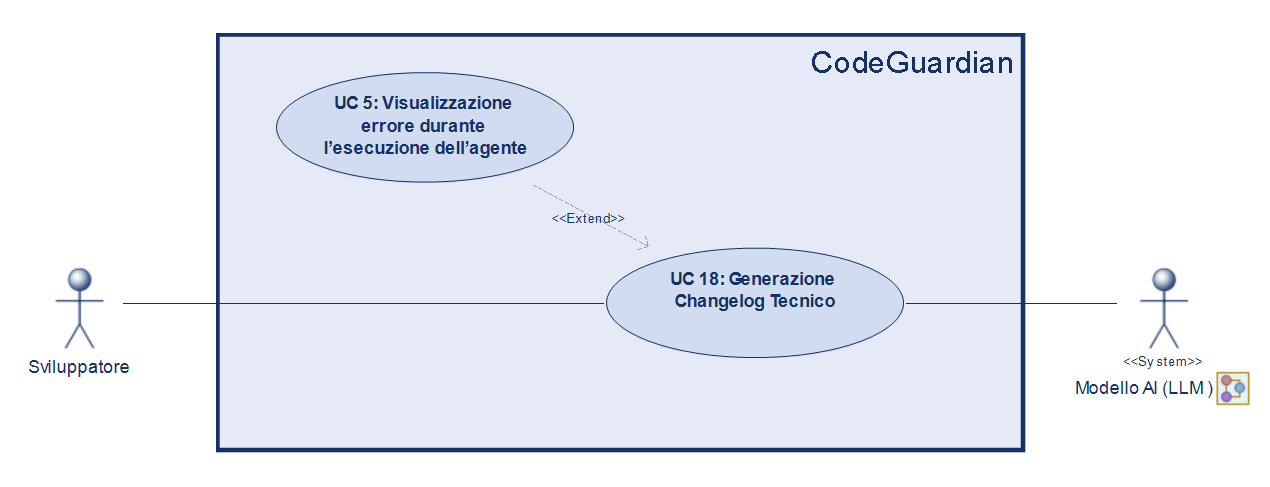
\includegraphics[width=1\linewidth]{UML UC18.png}
    \caption{Use Case Generazione Changelog Tecnico}
    \label{fig:UC18}
\end{figure}

\begin{itemize}
    \item \textbf{\textit{Attore} Primario}: Sviluppatore.
    \item \textbf{\textit{Attori} Secondari}: Modello AI (\textit{LLM}).
    \item \textbf{Trigger}: Richiesta esplicita dello sviluppatore di generare un \textit{Changelog} Tecnico e conclusione con successo della fase di recupero, filtraggio e validazione dei dati dello \textit{Sprint} (UC 15).
    \item \textbf{Precondizioni}: 
        \begin{itemize}
            \item L'Agente Changelog dispone del set di dati delle \textit{User Stories} validato e privo di ambiguità bloccanti (superamento di UC 16 e UC 17).
            \item I parametri di configurazione del \textit{Repository} sono accessibili.
        \end{itemize}
    \item \textbf{Postcondizioni}: Viene generato un report tecnico pronto per la revisione umana (UC 4) o per l'esportazione diretta (UC 6).
    \item \textbf{Scenario Principale}:
        \begin{enumerate}
            \item L'Agente analizza il set di dati aggregato e raggruppa le lavorazioni in macro-categorie tecniche standard (es. \texttt{Added}, \texttt{Changed}, \texttt{Fixed}, \texttt{Deprecated}).
            \item Per ogni \textit{User Story}, l'Agente interroga l'\textit{LLM} inviando i dettagli tecnici e i criteri di accettazione, richiedendo una sintesi in linguaggio ingegneristico asciutto e privo di ridondanze commerciali.
            \item L'Agente genera la struttura del documento formattando l'output con un formato di \textit{Markdown}.
            \item L'Agente inserisce per ogni voce i collegamenti ipertestuali e gli identificativi (ID) corrispondenti ai \textit{Ticket} di origine sul Sistema di Task Management.
            \item La bozza del file prodotto viene memorizzata in attesa di essere validata.
        \end{enumerate}
    \item \textbf{Scenario Alternativo}: 
    \begin{itemize}
    \item L'Agente non riceve risposta dall'\textit{LLM} entro il tempo limite oppure riceve un output la cui struttura non è parsabile dal sistema, l'elaborazione viene interrotta e il flusso passa all'UC 5 per la visualizzazione dell'errore.
\end{itemize}
\end{itemize}

\subsubsection{UC 19: Generazione \textit{Changelog} di Business (Dev-to-Client)}\label{uc:19}
L'Agente esegue una traduzione semantica per trasformare il gergo tecnico in benefici tangibili per gli \textit{Stakeholder}.

\begin{figure}[htbp]
    \centering
    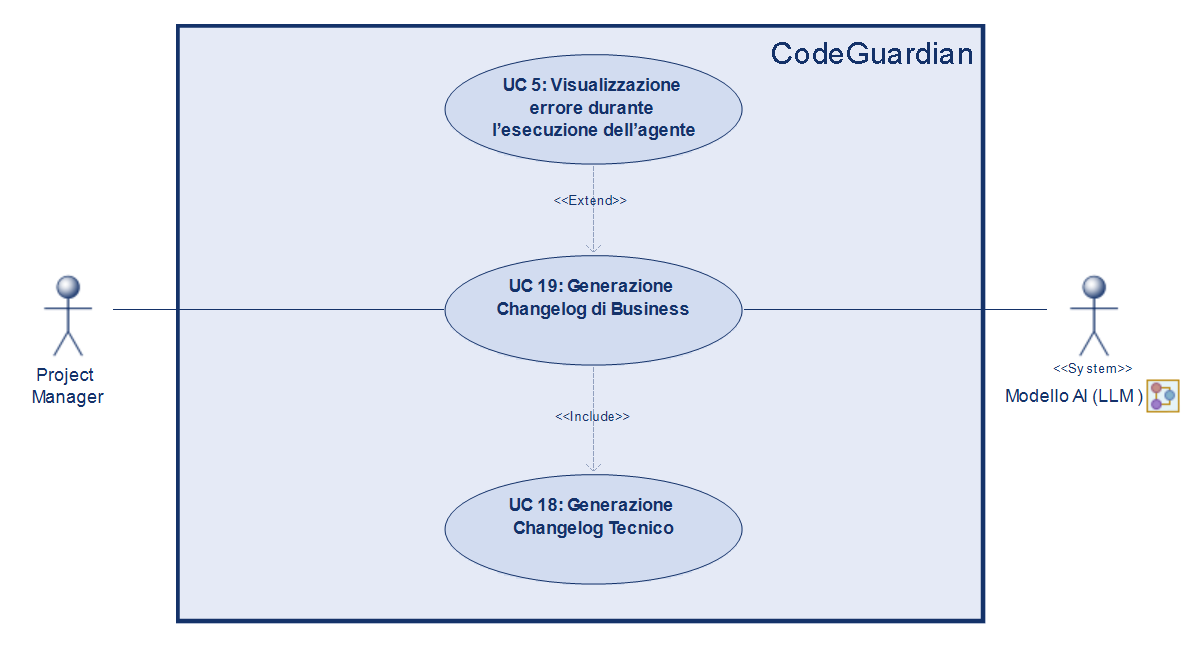
\includegraphics[width=1\linewidth]{UML UC19.png}
    \caption{Use Case Generazione Changelog di Business}
    \label{fig:UC19}
\end{figure}

\begin{itemize}
\item \textbf{\textit{Attore} Primario}: \textit{Project Manager}.
\item \textbf{\textit{Attori} Secondari}: Modello AI (\textit{LLM}).
\item \textbf{Trigger}: Richiesta esplicita del \textit{Project Manager} di generare un \textit{Changelog} di Business, dopo la creazione del \textit{Changelog} Tecnico.
\item \textbf{Precondizioni}: 
        \begin{itemize}
            \item L'Agente Changelog dispone del set di dati delle \textit{User Stories} validato e privo di ambiguità bloccanti (superamento di UC 16 e UC 17).
            \item I parametri di configurazione del \textit{Repository} sono accessibili.
        \end{itemize}
\item \textbf{Postcondizioni}: È disponibile un documento di \textit{Changelog} orientato al business pronto per la revisione umana (UC 4) o per l'esportazione diretta (UC 6).
\item \textbf{Scenario Principale}: 
\begin{enumerate}
            \item L'Agente riceve in input il testo del \textit{Changelog} Tecnico prodotto dall'UC 18.
            \item L'Agente interroga l'\textit{LLM} inviando il testo tecnico e applicando le direttive sul tono e sull'audience a cui si riferisce il documento.
            \item L'Agente analizza le singole voci tecniche (es. modifiche a database, refactoring, patch di sicurezza) e ne estrae l'equivalente impatto funzionale.
            \item L'Agente traduce i termini specialistici in benefici tangibili per l'utente finale, eliminando i dettagli implementativi di basso livello, poco rilevanti e poco comprensibili per il Cliente.
            \item L'Agente struttura la bozza del report di business e la memorizza, pronta per la validazione umana (UC 4).
\end{enumerate}
    \item \textbf{Scenario Alternativo}: 
    \begin{itemize}
    \item Il Changelog Tecnico non è stato genearto in precedenza al passo 1, quindi Il sistema invoca automaticamente la generazione del Changelog Tecnico (Inclusione UC 18).
    \item L'Agente non riceve risposta dall'\textit{LLM} entro il tempo limite oppure riceve un output la cui struttura non è parsabile dal sistema, l'elaborazione viene interrotta e il flusso passa all'UC 5 per la visualizzazione dell'errore.
\end{itemize}
    \item \textbf{Inclusioni}: 
    \begin{itemize}
    \item UC 18: Generazione Changelog Tecnico.
\end{itemize}
\end{itemize}

\newpage

\section{Requisiti}

I requisiti riportati in questa sezione sono stati derivati dai \textit{Casi d'Uso} descritti nel capitolo 3 e dalle indicazioni emerse dagli incontri con il \textbf{Proponente}. In particolare, il perimetro del progetto è stato
chiarito come sviluppo di agenti specializzati da integrare in
un'architettura già esistente, e non come realizzazione di una nuova
architettura completa ad agenti.

\subsection{Requisiti funzionali}
\begingroup
\renewcommand{\arraystretch}{1.3}

\begin{xltabular}{\textwidth}{|c|c|D|F|}

    \hline
    \textbf{Codice} & \textbf{Priorità} & \textbf{Descrizione} & \textbf{Fonti} \\ 
    \hline
    \endfirsthead

    \hline
    \textbf{Codice} & \textbf{Priorità} & \textbf{Descrizione} & \textbf{Fonti} \\ 
    \hline
    \endhead

    RF.0 & Obbligatorio & Il sistema deve consentire all'utente di inserire, convalidare e memorizzare in modo sicuro i token di accesso personali necessari per l'integrazione con i servizi esterni (\textit{Repository Git} e Sistema di Task Management). & UC 0 \\ \hline
    RF.1 & Obbligatorio & Il sistema deve consentire all'utente di selezionare il \textit{Repository Git} da utilizzare come contesto di esecuzione degli agenti, specificando anche il riferimento di base desiderato tra branch e \textit{Commit} specifico. & UC 1 \\ \hline
    RF.2 & Desiderabile & L'utente può utilizzare come riferimento del \textit{Repository Git} una \textit{Pull Request} specifica. & UC 1 
    \\ \hline
    RF.3 & Obbligatorio & Il sistema deve mostrare un messaggio di avviso all'utente qualora il \textit{repository} o l'ambito di analisi selezionato contenga codice sorgente scritto in linguaggi non supportati. & UC 1 
    \\ \hline
    RF.4 & Obbligatorio & Il sistema deve consentire all'utente di selezionare l’ambito di analisi, scegliendo uno o più file o directory del Repository. & UC 2 \\ 
    \hline
    RF.5 & Desiderabile &Il sistema deve mostrare un messaggio di errore e impedire l'avvio dell'agente qualora l'ambito di analisi selezionato (numero di file o volume di righe di codice) ecceda i limiti dimensionali entro i quali il modello \textit{LLM} garantisce performance affidabili. & UC 2, 5 \\ 
    \hline
    RF.6 & Desiderabile & Se supportato dalla configurazione del sistema, il sistema deve consentire la selezione dell’intero Repository come ambito di analisi. & UC 2 \\ 
    \hline
    RF.7 & Obbligatorio & Il sistema deve consentire all'utente di visualizzare il report prodotto dall’agente, includendo almeno criticità rilevate, suggerimenti proposti e file coinvolti. & UC 3 \\ 
    \hline
    RF.8 & Obbligatorio & Il sistema deve consentire all'utente di validare, modificare o rifiutare manualmente una proposta generata da un agente prima della sua eventuale applicazione. & UC 4 \\ 
    \hline
    RF.9 & Obbligatorio & Il sistema deve mostrare un messaggio di errore esplicativo in caso di fallimento durante l’esecuzione di un agente, indicando, ove possibile, una possibile azione correttiva. & UC 5, 15 \\ 
    \hline
    RF.10 & Desiderabile & Il sistema deve bloccare l'esecuzione di un agente e delegare la visualizzazione di un messaggio d'errore qualora la richiesta superi i limiti di utilizzo API imposti. & UC 5 \\ 
    \hline
    RF.11 & Desiderabile & Il sistema deve interrompere l'esecuzione di un agente e mostrare un messaggio di errore all'utente qualora il tempo di elaborazione del modello AI (LLM) superi la soglia massima consentita (Timeout di risposta). & UC 5, 8, 9, 12, 13, 14, 18, 19 \\ 
    \hline
    RF.12 & Obbligatorio & Il sistema deve consentire l’esportazione del report generato da un agente in formato PDF. & UC 6 \\ 
    \hline
    RF.13 & Opzionale & Il sistema deve mantenere un archivio storico dei report generati, consentendo all'utente di selezionare un report passato ai fini dell'esportazione. & UC 6 \\ 
    \hline
    RF.14 & Obbligatorio & Il sistema deve generare o aggiornare il file README.md del progetto in modo coerente con lo stato corrente del Repository e in lingua inglese. & UC 7 \\ 
    \hline
    RF.15 & Opzionale & Il sistema deve permettere all'utente di impostare un modello di stile personalizzato per il file README.md. & UC 7 \\ 
    \hline
    RF.16 & Obbligatorio & Il sistema deve generare o aggiornare la documentazione inline del codice (JSDoc) per gli elementi sorgente supportati. & UC 8 \\ 
    \hline
    RF.17 & Obbligatorio & Il sistema deve correggere documentazione inline esistente quando questa non è più coerente con il codice. & UC 8 \\ 
    \hline
    RF.18 & Desiderabile & Il sistema deve segnalare allo Sviluppatore i casi in cui la logica risulti troppo complessa per una documentazione automatica affidabile. & UC 8 \\ 
    \hline
    RF.19 & Obbligatorio & Il sistema deve generare o aggiornare la documentazione delle API del progetto. & UC 9\\
    \hline
    RF.20 & Obbligatorio & Il sistema deve riconoscere quando le modifiche apportate al codice sorgente non alterano il comportamento, i componenti o gli endpoint analizzati, terminando l'esecuzione senza generare nuove proposte di aggiornamento documentale. & UC 7, 8, 9\\
    \hline
    RF.21 & Obbligatorio & Il sistema deve eseguire un'analisi di sicurezza del codice alla ricerca di vulnerabilità riconducibili alle categorie \textit{OWASP} rilevanti. & UC 10 \\
    \hline
    RF.22 & Obbligatorio & Il sistema deve associare ogni vulnerabilità rilevata almeno al file interessato e, se disponibile, alla porzione di codice coinvolta. & UC 10 \\
    \hline
    RF.23 & Obbligatorio & Il sistema deve classificare le vulnerabilità rilevate indicando almeno categoria \textit{OWASP} e livello di gravità. & UC 10 \\
    \hline
    RF.24 & Obbligatorio & Il sistema deve verificare la conformità del codice rispetto alle policy di sviluppo sicuro definite dal team nel file CLAUDE.md. & UC 11 \\
    \hline
    RF.25 & Obbligatorio & Il sistema deve generare suggerimenti di remediation per vulnerabilità o violazioni di policy rilevate. & UC 12 \\ 
    \hline
    RF.26 & Obbligatorio & Quando la problematica è sufficientemente localizzata nel codice, il sistema deve poter generare uno snippet di codice correttivo da sottoporre a validazione umana. & UC 13 \\
    \hline
    RF.27 & Obbligatorio & Quando non è possibile proporre in modo affidabile uno snippet locale, il sistema deve generare una descrizione testuale della remediation da effettuare. & UC 14 \\ 
    \hline
    RF.28 & Obbligatorio & Il sistema deve recuperare, da un sistema di Task Management esterno, le User Stories e i task completati relativi a uno specifico Sprint. & UC 15 \\
    \hline
    RF.29 & Obbligatorio & Il sistema deve filtrare le User Stories e i task completati relativi a uno specifico Sprint. & UC 15 \\
    \hline
    RF.30 & Obbligatorio & Il sistema deve poter identificare lo Sprint di riferimento attraverso la label contenente il codice dello Sprint associata alle issue o ai task. & UC 15, Verbale esterno 2026/04/24 \\
    \hline
    RF.31 & Obbligatorio & Il sistema deve estrarre dai task selezionati almeno titolo, descrizione, criteri di accettazione e commenti rilevanti. & UC 15 \\ 
    \hline
    RF.32 & Obbligatorio & Il sistema deve rilevare task con metadati insufficienti e segnalarli all’utente, escludendoli dal flusso di generazione automatica del \textit{Changelog}. & UC 16 \\
    \hline
    RF.33 & Opzionale & Il sistema deve rilevare ambiguità o incoerenze tra la documentazione della User Story e i dati tecnici associati, segnalandole all’utente per risoluzione manuale. & UC 17 \\
    \hline
    RF.34 & Obbligatorio & Il sistema deve generare un \textit{Changelog} tecnico orientato allo sviluppo, strutturato a partire dai task validati dello Sprint. & UC 18 \\
    \hline
    RF.35 & Desiderabile &  Il \textit{Changelog} tecnico deve includere i collegamenti ipertestuali e gli identificativi dei ticket di origine, quando tali informazioni sono disponibili. & UC 18 \\
    \hline
    RF.36 & Obbligatorio & Il sistema deve generare un \textit{Changelog} orientato al business, comprensibile a stakeholder non tecnici, a partire dal \textit{Changelog} tecnico, genearto dai dati validati dello Sprint. & UC 18,19 \\
    \hline

\end{xltabular}
\endgroup


\subsection{Requisiti qualitativi}

\begingroup
\renewcommand{\arraystretch}{1.3}

\begin{xltabular}{\textwidth}{|c|c|D|F|}

    \hline
    \textbf{Codice} & \textbf{Priorità} & \textbf{Descrizione} & \textbf{Fonti} \\ 
    \hline
    \endfirsthead

    \hline
    \textbf{Codice} & \textbf{Priorità} & \textbf{Descrizione} & \textbf{Fonti} \\ 
    \hline
    \endhead

    RQ.0 & Obbligatorio & Il sistema deve adottare un approccio \textit{Human-in-the-loop}, mantenendo il controllo umano nella validazione degli output prodotti dagli agenti. & UC 4, Verbale esterno 2026/03/23 \\ 
    \hline
    RQ.1 & Obbligatorio &  Gli output prodotti dagli agenti devono risultare utili al miglioramento del codice, ad esempio tramite segnalazioni, suggerimenti testuali, frammenti di codice o proposte di soluzione. & Verbale esterno 2026/03/23 \\
    \hline
    RQ.2 & Desiderabile & Il sistema deve minimizzare i falsi positivi nella generazione della documentazione, evitando di proporre aggiornamenti per modifiche al codice puramente stilistiche o marginali. & UC 7, 8, 9 \\
    \hline
    RQ.3 & Obbligatorio & Devono essere definite modalità di test e validazione per gli agenti sviluppati e per i modelli o servizi utilizzati. & Verbale esterno 2026/03/23 \\
    \hline
    RQ.4 & Obbligatorio & L’output dell’Agente Changelog destinato al cliente o agli stakeholder deve essere scritto in modo comprensibile dal lato business, evitando tecnicismi non necessari. & Verbale esterno 2026/04/24 \\
    \hline
    RQ.5 & Desiderabile & l tempo di attesa per l'esecuzione di un agente su un ambito di analisi ristretto (es. file singolo o porzione di codice locale) non dovrebbe superare una soglia temporale ragionevole (es. 2-3 minuti), al fine di non ostacolare il flusso di lavoro dell'utente. & Capitolato C2 \\
    \hline
    
\end{xltabular}
\endgroup


\subsection{Requisiti di vincolo}

\begingroup
\renewcommand{\arraystretch}{1.3}

\begin{xltabular}{\textwidth}{|c|c|D|F|}

    \hline
    \textbf{Codice} & \textbf{Priorità} & \textbf{Descrizione} & \textbf{Fonti} \\ 
    \hline
    \endfirsthead

    \hline
    \textbf{Codice} & \textbf{Priorità} & \textbf{Descrizione} & \textbf{Fonti} \\ 
    \hline
    \endhead

    RV.0 & Obbligatorio & Il progetto prevede lo sviluppo, da parte del team, di un Orchestratore centrale che invoca gli agenti e fa da itermediario tra utenti e agenti. & Verbale esterno 2026/06/08 \\
    \hline
    RV.1 & Obbligatorio & Il progetto non deve prevedere l’addestramento di nuovi modelli, ma l’integrazione di modelli o servizi tramite API. & Verbale esterno 2026/03/23 \\
    \hline
    RV.2 & Obbligatorio & Il sistema deve poter operare sui Repository di esempio e sul codice reso disponibile dal Proponente per i test. & Verbale esterno 2026/03/23 \\
    \hline
    RV.3 & Obbligatorio & Il sitema deve poter operare a pieno anche su Repository privati, oltre a quelli pubblici. & Verbale esterno 2026/06/08 \\
    \hline
    RV.4 & Obbligatorio & Il sistema deve basarsi sull’analisi di Repository software e sulla produzione di output documentazione e remediation coerenti con il perimetro del progetto Code Guardian. &  Capitolato C2 \\
    \hline
    RV.5 & Desiderabile & Il sistema dovrebbe prevedere un meccanismo di limitazione di utilizzo a livello di configurazione per tutelare il budget API. &  Verbale interno 2026/06/02 \\
    \hline
    RV.6 & Obbligatorio & Il sistema deve supportare e garantire l'analisi per Repository contenenti codice sorgente scritto nei linguaggi TypeScript, JavaScript e Python. &  Verbale esterno 2026/06/03 \\
    \hline
    
\end{xltabular}
\endgroup

\subsection{Requisiti di sicurezza}

\begingroup
\renewcommand{\arraystretch}{1.3}

\begin{xltabular}{\textwidth}{|c|c|D|F|}

    \hline
    \textbf{Codice} & \textbf{Priorità} & \textbf{Descrizione} & \textbf{Fonti} \\ 
    \hline
    \endfirsthead

    \hline
    \textbf{Codice} & \textbf{Priorità} & \textbf{Descrizione} & \textbf{Fonti} \\ 
    \hline
    \endhead

    RS.0 & Obbligatorio & Il sistema deve memorizzare i token di accesso e le credenziali fornite dall'utente esclusivamente in formato cifrato all'interno del proprio livello di persistenza. & UC 0 \\
    \hline
    RS.1 & Obbligatorio & Le eventuali modifiche proposte al codice o ai file del Repository non devono essere applicate senza validazione umana preventiva. & Verbale esterno 2026/03/23 \\
    \hline
    RS.2 & Obbligatorio &  I risultati dell’analisi di sicurezza devono riportare almeno il tipo di problematica rilevata, il livello di gravità e, se disponibile, il riferimento al file o alla porzione di codice interessata. & UC 10 \\
    \hline
    RS.3 & Obbligatorio & L’accesso a Repository, sistemi di Task Management e servizi esterni deve avvenire tramite credenziali, token o chiavi API validi e coerenti con i permessi richiesti dall’operazione. & UC 0, 15 \\
    \hline
    RS.4 & Desiderabile & Il sistema dovrebbe interfacciarsi con i servizi LLM esterni utilizzando policy o tier di servizio API che garantiscano che il codice sorgente analizzato non venga trattenuto o utilizzato per l'addestramento di modelli di terze parti. & Capitolato C2 \\
    \hline
    
\end{xltabular}
\endgroup

\newpage

\section{Tracciamento}

Questa sezione illustra il tracciamento bidirezionale tra le fonti originali (Casi d'Uso, Verbali, Capitolato) e i requisiti derivati. Le tabelle seguenti mappano questa corrispondenza in modo sistematico, garantendo coerenza e facilitandone la consultazione.

\subsection{Tracciamento Fonte - Requisiti}

\begingroup
\renewcommand{\arraystretch}{1.3}
\begin{xltabular}{\textwidth}{|c|X|}
    \hline
    \textbf{Fonte} & \textbf{Requisiti} \\ 
    \hline
    \endfirsthead

    \hline
    \textbf{Fonte} & \textbf{Requisiti} \\ 
    \hline
    \endhead

    \hyperref[uc:1]{UC 1} & RF.1 \\ \hline
    \hyperref[uc:2]{UC 2} & RF.4, RF.6 \\ \hline
    \hyperref[uc:3]{UC 3} & RF.7 \\ \hline
    \hyperref[uc:4]{UC 4} & RF.8, RQ.0 \\ \hline
    \hyperref[uc:5]{UC 5} & RF.9 \\ \hline
    \hyperref[uc:6]{UC 6} & RF.12 \\ \hline
    \hyperref[uc:7]{UC 7} & RF.14, RF.20, RQ.2 \\ \hline
    \hyperref[uc:8]{UC 8} & RF.16, RF.17, RF.18, RF.20, RQ.2 \\ \hline
    \hyperref[uc:9]{UC 9} & RF.19, RF.20, RQ.2 \\ \hline
    \hyperref[uc:10]{UC 10} & RF.21, RF.22, RF.23, RS.2 \\ \hline
    \hyperref[uc:11]{UC 11} & RF.24 \\ \hline
    \hyperref[uc:12]{UC 12} & RF.25 \\ \hline
    \hyperref[uc:13]{UC 13} & RF.26 \\ \hline
    \hyperref[uc:14]{UC 14} & RF.27 \\ \hline
    \hyperref[uc:15]{UC 15} & RF.15, 28, RF.30, RF.31, RS.3 \\ \hline
    \hyperref[uc:16]{UC 16} & RF.32 \\ \hline
    \hyperref[uc:17]{UC 17} & RF.33 \\ \hline
    \hyperref[uc:18]{UC 18} & RF.34, RF.35 \\ \hline
    \hyperref[uc:19]{UC 19} & RF.36 \\ \hline
    Capitolato C2 & RV.4 \\ \hline
    Verbale esterno 2026/03/23 & RQ.0, RQ.1, RQ.3, RV.1, RV.2, RS.1 \\ \hline
    Verbale esterno 2026/04/24 & RF.30, RQ.4 \\ \hline
    Verbale esterno 2026/06/08 & RV.0, RV.3 \\ \hline

\end{xltabular}
\endgroup

\newpage

\subsection{Tracciamento Requisito - Fonti}

\begingroup
\renewcommand{\arraystretch}{1.3}
\begin{xltabular}{\textwidth}{|c|X|}
    \hline
    \textbf{Requisito} & \textbf{Fonti} \\ 
    \hline
    \endfirsthead

    \hline
    \textbf{Requisito} & \textbf{Fonti} \\ 
    \hline
    \endhead

    RF.1 & \hyperref[uc:1]{UC 1} \\ \hline
    RF.4 & \hyperref[uc:2]{UC 2} \\ \hline
    RF.6 & \hyperref[uc:2]{UC 2} \\ \hline
    RF.7 & \hyperref[uc:3]{UC 3} \\ \hline
    RF.8 & \hyperref[uc:4]{UC 4} \\ \hline
    RF.9 & \hyperref[uc:5]{UC 5}, \hyperref[uc:15]{UC 15} \\ \hline
    RF.12 & \hyperref[uc:6]{UC 6} \\ \hline
    RF.14 & \hyperref[uc:7]{UC 7} \\ \hline
    RF.16 & \hyperref[uc:8]{UC 8} \\ \hline
    RF.17 & \hyperref[uc:8]{UC 8} \\ \hline
    RF.18 & \hyperref[uc:8]{UC 8} \\ \hline
    RF.19 & \hyperref[uc:9]{UC 9} \\ \hline
    RF.20 & \hyperref[uc:7]{UC 7}, \hyperref[uc:8]{UC 8}, \hyperref[uc:9]{UC 9} \\ \hline
    RF.21 & \hyperref[uc:10]{UC 10} \\ \hline
    RF.22 & \hyperref[uc:10]{UC 10} \\ \hline
    RF.23 & \hyperref[uc:10]{UC 10} \\ \hline
    RF.24 & \hyperref[uc:11]{UC 11} \\ \hline
    RF.25 & \hyperref[uc:12]{UC 12} \\ \hline
    RF.26 & \hyperref[uc:13]{UC 13} \\ \hline
    RF.27 & \hyperref[uc:14]{UC 14} \\ \hline
    RF.28 & \hyperref[uc:15]{UC 15} \\ \hline
    RF.30 & \hyperref[uc:15]{UC 15}, Verbale esterno 2026/04/24 \\ \hline
    RF.31 & \hyperref[uc:15]{UC 15} \\ \hline
    RF.32 & \hyperref[uc:16]{UC 16} \\ \hline
    RF.33 & \hyperref[uc:17]{UC 17} \\ \hline
    RF.34 & \hyperref[uc:18]{UC 18} \\ \hline
    RF.35 & \hyperref[uc:18]{UC 18} \\ \hline
    RF.36 & \hyperref[uc:19]{UC 19} \\ \hline
    RQ.0 & \hyperref[uc:4]{UC 4}, Verbale esterno 2026/03/23 \\ \hline
    RQ.1 & Verbale esterno 2026/03/23 \\ \hline
    RQ.2 & \hyperref[uc:7]{UC 7}, \hyperref[uc:8]{UC 8}, \hyperref[uc:9]{UC 9} \\ \hline
    RQ.3 & Verbale esterno 2026/03/23 \\ \hline
    RQ.4 & Verbale esterno 2026/04/24 \\ \hline
    RV.0 & Verbale esterno 2026/06/08\\ \hline
    RV.1 & Verbale esterno 2026/03/23 \\ \hline
    RV.2 & Verbale esterno 2026/06/08 \\ \hline
    RV.3 & Verbale esterno 2026/03/23 \\ \hline
    RV.4 & Capitolato C2 \\ \hline
    RS.1 & Verbale esterno 2026/03/23 \\ \hline
    RS.2 & \hyperref[uc:10]{UC 10} \\ \hline
    RS.3 & \hyperref[uc:15]{UC 15} \\ \hline

\end{xltabular}
\endgroup

\end{document}
